\documentclass[a4paper,12pt,oneside]{book}
\usepackage[ngerman]{babel}
\usepackage[utf8]{inputenc}
\usepackage[T1]{fontenc}
\catcode`\_=12 % change catcode of "_" to "other" (no. 12)
\usepackage{csquotes}
\usepackage{graphicx}
\usepackage{subfigure}
\usepackage{dirtree}
\usepackage{svg}
\usepackage{amsmath}

\setcounter{secnumdepth}{4}
\setcounter{tocdepth} {2}
\setcounter{secnumdepth} {3}
\usepackage{marvosym}
\usepackage{fancyhdr}
\pagestyle{fancy}
\usepackage[subfigure]{tocloft}
\renewcommand{\cftfigfont}{Abbildung }
\renewcommand{\cfttabfont}{Table }
\renewcommand{\cftfigaftersnum}{ :}
\renewcommand{\cfttabaftersnum}{ :}
\usepackage{subfigure}
\usepackage[T1]{fontenc}
\renewcommand{\sectionmark}[1]{\markright{\thesection\ #1}}
\fancyhf{} % supprime les en-t\^etes et pieds pr\'ed\'efinis
\fancyhead[LE,RO]{\bfseries\thepage}% Left Even, Right Odd
\fancyhead[LO]{\bfseries\rightmark} % Left Odd
\fancyhead[RE]{\bfseries\leftmark} % Right Even
\renewcommand{\headrulewidth}{0.5pt}% filet en haut de page
\addtolength{\headheight}{0.5pt} % espace pour le filet
\renewcommand{\footrulewidth}{0pt} % pas de filet en bas
\fancypagestyle{plain}{ % pages de tetes de chapitre
	\fancyhead{} % supprime l'entete
	\renewcommand{\headrulewidth}{0pt} % et le filet
	\fancyfoot[C]{\bfseries\thepage} %contient uniquement le num de page en pieds de page
}

\usepackage{color}
\usepackage{titlesec}
\titlespacing{\section}{0pt}{0.3cm}{0.3cm}
\titlespacing{\subsection}{0pt}{0.3cm}{0.3cm}
\titlespacing{\subsubsection}{0pt}{0.3cm}{0.3cm}
\definecolor{gris10}{gray}{0.9} %si on veut utiliser une nuance de la couleur grise
\definecolor{bleufonce}{rgb}{0,0,0.55}
\usepackage[top=25mm, bottom=25mm, left=25mm , right=25mm]{geometry}
\linespread{1.4} %interligne
%\setlength{\parindent}{0 pt} %pas d'indentation
\setlength{\parskip}{1.5ex plus 1ex minus 0.5ex}
\addto\captionsfrench{%
	\renewcommand{\listfigurename}{Liste des figures}%
}
\setcounter{tocdepth} {2}
\setcounter{secnumdepth} {3}
\usepackage{listings}


\definecolor{dkgreen}{rgb}{0,0.6,0}
\definecolor{gray}{rgb}{0.5,0.5,0.5}
\definecolor{mauve}{rgb}{0.58,0,0.82}

\lstset{frame=tb,
	language=java,
	aboveskip=3mm,
	belowskip=3mm,
	showstringspaces=false,
	columns=flexible,
	basicstyle={\small\ttfamily},
	numbers=none,
	numberstyle=\tiny\color{gray},
	keywordstyle=\color{blue},
	commentstyle=\color{dkgreen},
	stringstyle=\color{mauve},
	breaklines=true,
	breakatwhitespace=true,
	tabsize=3
}

\definecolor{maroon}{rgb}{0.5,0,0}
\definecolor{darkgreen}{rgb}{0,0.5,0}
\lstdefinelanguage{XML}
{
	basicstyle=\ttfamily,
	morestring=[s]{"}{"},
	morecomment=[s]{?}{?},
	morecomment=[s]{!--}{--},
	commentstyle=\color{darkgreen},
	moredelim=[s][\color{black}]{>}{<},
	moredelim=[s][\color{red}]{\ }{=},
	stringstyle=\color{blue},
	identifierstyle=\color{maroon}
}

\usepackage{fancyhdr}
\pagestyle{fancy}
\renewcommand{\chaptermark}[1]{\markboth{#1}{}}
\renewcommand{\sectionmark}[1]{\markright{\thesection\ #1}}
\fancyhf{} % supprime les en-t\^etes et pieds pr\'ed\'efinis
\fancyhead[LE,RO]{\bfseries\thepage}% Left Even, Right Odd
\fancyhead[LO]{\bfseries\rightmark} % Left Odd
\fancyhead[RE]{\bfseries\leftmark} % Right Even
\renewcommand{\headrulewidth}{0.5pt}% filet en haut de page
\addtolength{\headheight}{0.5pt} % espace pour le filet
\renewcommand{\footrulewidth}{0pt} % pas de filet en bas
\fancypagestyle{plain}{ % pages de tetes de chapitre
	\fancyhead{} % supprime l'entete
	\renewcommand{\headrulewidth}{0pt} % et le filet
	\fancyfoot[C]{\bfseries\thepage} %contient uniquement le num de page en pieds de page
}
\title{Wissenschaftliche-Vertiefung-Ausarbeitung}
\date{01.07.2019} 
\author{Mohamed Karim Swissi  }
\begin{document}
	
\begin{titlepage}
	\thispagestyle{empty}
	\begin{center}
		Westfälische Hochschule Gelsenkirchen
		
		
		
\includegraphics[scale=0.8, width=6cm, height=4cm]{w-hs_pagelogo.png}
		
		Fachbereich Informatik und Kommunikation 
		
		
		\vskip 2cm
		\centerline{\Large{\textbf{Wissenschaftliche Vertiefung }}}
		
		\vskip 0.5cm
		\centerline{\Large{\textbf{  }}}
		
		%\centerline{\footnotesize{de} \small{\textbf{l'Ecole Nationale d'Ing\'enieurs de Tunis}}}
		
		
		\vskip 1cm
		
		\fbox{
			\begin{minipage}{10cm}
				\vspace{0.5cm}
				\begin{center}
					{\LARGE  {\textbf {\textit{Testautomatisierung :  \newline Test-C Plattform}}}}
					
				\end{center}
				\vspace{0.1cm}
			\end{minipage}
		}
		\vskip 1cm
		\centerline{Vorgelegt von:}
		\vskip 0.4cm
		\centerline{\Large \textbf{Mohamed Karim Swissi}}
		\vskip 0.4cm
		\centerline{\Large \textbf{Matrikel-Nr: 201610895}}
		
		
		
		\vskip 1cm
		
		
		\centerline{Betreuender Professor:}
		\vskip 0.4cm
		\begin{center}
			\large \textbf{Prof. Dr. Ulrike Griefahn} \\
		\end{center}
		
		\vskip 0.4cm
		
		
		
		\vskip 1cm
		\centerline{Wintersemester 2019/2020}
		
	\end{center}
	
\end{titlepage}
\newpage
	
	
\tableofcontents
\newpage
\addcontentsline{toc}{section}{Abbildungsverzeichnis}
\listoffigures
\newpage
\addcontentsline{toc}{section}{listings}
\lstlistoflistings
\newpage
\chapter{Motivation}
Bei der Computerprogrammierung handelt es sich beim 'unit testing' um eine Software-Testmethode, mit der einzelne Einheiten des Quellcodes,  Verwendungsverfahren und Betriebsverfahren getestet werden, um festzustellen, ob sie zur Verwendung geeignet sind.
\newline
Unit-Tests sind typischerweise automatisierte Tests, die von Softwareentwicklern geschrieben und ausgeführt werden, um sicherzustellen, dass ein Teil einer Anwendung dem Design entspricht und sich wie vorgesehen verhält.
\newline
Beim Testen von Software wird bei der Testautomatisierung eine spezielle Software (unabhängig von der getesteten Software) verwendet, um die Ausführung von Tests und den Vergleich der tatsächlichen Ergebnisse mit den prognostizierten Ergebnissen zu steuern.
\newline
In diesem Projekt wird eine andere Art der Verwendung eines solchen Automatisierungsframeworks erörtert.
\chapter{Einleitung}
\section{Aufgabenbeschreibung}

Im Rahmen dieses wissenschaftlichen Vertiefungsprojekts wird ein, wird ein Testplattform basierend auf Docker 'Virtualisierung' , Unit Tests und Automatisierung entwickelt.
\newline
Mit dieser Testplattform können die Schüler ihre Aufgabenblätter-Lösungen testen, um einen Testbericht zu erhalten.
\section{Herangehensweise}
In dieser Ausarbeitung werden die Techniken und Technologien vorgestellt, die in diesem Projekt verwendet werden. Daher wurde das Konzept des Code-Testens erläutert. Ebenso wird das in diesem Projekt verwendete Unit-Test-System besprochen. Anschließend werden die Rolle des Jenkins-Tools im Projekt und die Bedeutung dieses Tools für die Automatisierung des Testprozesses erläutert, dann folgt eine ausführliche Erläuterung der Verwendung von Docker im Projekt. Abschließend eine Erläuterung von Git-Hosting und Jgit, die einen der wichtigsten Teile des Projekts darstellen.
\newline
Im Hauptabschnitt wird dann die Erstellung der Testplattform erläutert. Die Architektur wird detailliert beschrieben und anschließend werden die Komponenten des Projekts separat besprochen. Außerdem werden die Installationsanweisungen und die Verwendung der Testplattform vorgestellt.

\chapter{Grundlagen}
\section{Code Testing}
Beim Softwaretesten wird ein Programm oder eine Anwendung ausgeführt, um die Fehler zu ermitteln und um zu überprüfen, ob die erforderlichen Bedingungen erfüllt sind.
\newline
Softwaretestverfahren können in 2 Gruppen unterteilt werden:Statisches und Dynamisches Testen.
\subsection{Manual testing( Statisches)}
Eine Softwaretesttechnik, bei der die Software getestet wird, ohne den Code auszuführen. Es besteht aus zwei Teilen:
\begin{itemize}
	\item Review - Wird normalerweise verwendet, um Fehler oder Unklarheiten in Dokumenten wie Anforderungen, Design, Testfällen usw. zu finden und zu beseitigen.
	\item Statische Analyse - Der von Entwicklern geschriebene Code wird (normalerweise mithilfe von Werkzeugen) auf strukturelle Fehler analysiert. 
\end{itemize}
\subsection{Automated Testing(Dynamisches)}
Beim dynamischen Testen wird die Software auf die Eingabewerte geprüft und werden die Ausgabewerte analysiert. Es gibt verschiedene Arten dynamischer Testtechniken: 
\begin{itemize}
	\item Unit Testing
	\item Integration Testing
	\item System Testing
	\item Acceptance Testing
\end{itemize}
In diesem Fall werden dynamische Tests verwendet, um die Programmieraufgaben der Studenten zu bewerten.

\chapter{Test-C Plattform}
\section{Einführung}
In diesem Abschnitt wird die Test C-Plattform detailliert beschrieben, wobei zunächst die Zusammensetzung der gesamten Programmarchitektur erörtert wird, wodurch die Programmkomponenten separat diskutiert werden können.Nach einer separaten Erläuterung der Programmkomponenten wird im Abschnitt (Installationsanleitung) genau erklärt, wie die Test-C-Plattform installiert und konfiguriert wird. Schließlich folgt ein Abschnitt, der die Verwendung des Projekts erläutert.

\section{Architektur}
\begin{figure}[h!]
	\begin{center}
		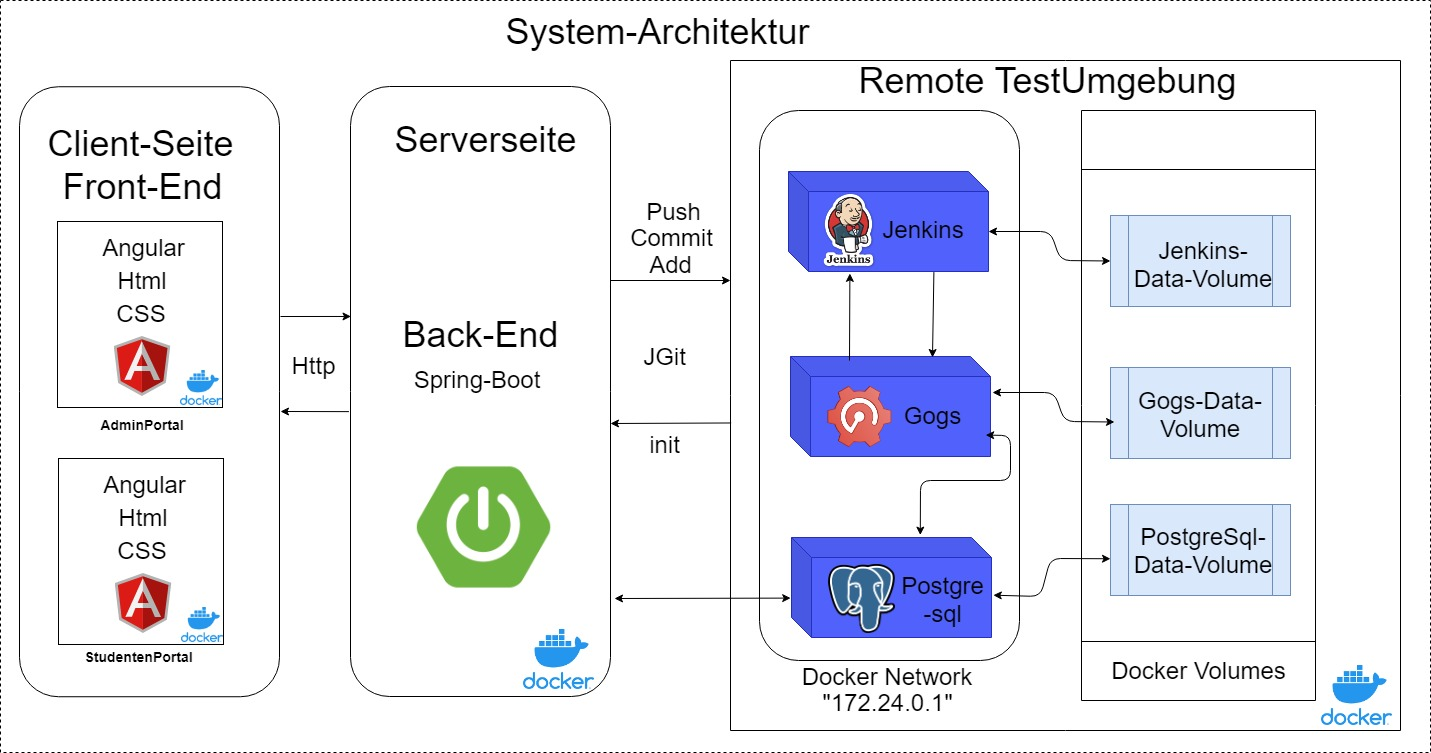
\includegraphics[width=17cm, height=14cm]{Test-C-Plattform-Arch.jpg}
		\caption{Architektur Test-C-Plattform } 
		\label{ Architektur Test-C-Plattform } 
	\end{center}
\end{figure}
Wie in der Abbildung 4.1 wird gezeigt, ist die Test-C-Plattformarchitektur in drei Hauptteile unterteilt: Client-Seite, Serverseite und Remote-TestUmgebung.
\newline
Die Wahl der Technologien beruhte auf ihrer Modernität und ihrer Verbreitung auf dem Arbeitsmarkt. In dem ersten Teil des Projekts (Client-Seite/Frontend) wurde die folgenden Techniken verwendet : Angular 7, NGX-Bootstrap, Html, Css. Im zweiten Teil des Projekts (Serverseite / BackEnd) wurden Maven und Spring Boot, Spring Security und Ldap bzw Spring Stack verwendet.Der dritte Teil enthält die Komponenten, die für die Durchführung des Testprozesses verantwortlich sind.
\newpage
Im folgenden Abschnitt wird jeder Teil der Architektur separat erklärt.
\newpage
\section{Client-Seite (Front-End)}
\begin{figure}[h!]
	\begin{center}
		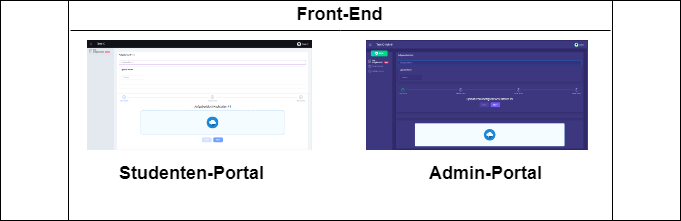
\includegraphics[width=14cm, height=6cm]{FrontEnd.png}
		\caption{Front-End } 
		\label{ Front-End } 
	\end{center}
\end{figure}
In diesem Projekt ist das Frontend in zwei Komponenten unterteilt: das Administrationsportal und das Studentenportal. Beide Portale wurden mit Angular 7, Html, Css und NGX-Bootstrap entwickelt.
\newline
Über das Administrationsportal kann der Admin Benutzer ein neues Aufgabenblatt erstellen. Dies bedeutet, dass ein virtueller Bereich für den Aufgabenblatttest erstellt wird, in dem die Studenten ihre Lösungen für Aufgaben testen können. Der Administrator kann alle Testdateien für jedes Aufgabenblatt in den entsprechenden Testbereich hochladen. Der Administrator hat auch einer Zugriff auf die Testbereiche. Jeder Testbereich ist mit dem Namen des zu testenden Aufgabenblatts gekennzeichnet. Für jeden Testbereich werden die spezifischen Testdateien angezeigt und der Administrator kann davon Dateien löschen oder andere hinzufügen.
Über das Studentenportal kann der Student die zu testende Lösungsdatei hochladen und dann an den Testbereich senden, der den Test automatisch durchführt und dem Studenten das Testergebnis anzeigt.
\section{Remote TestUmgebung}
Die Erklärung dieses Teils des Projekts ist vor der Erklärung des Mittelteils 'Serverseite' eine absichtliche Sache, damit der Leser einfach verstehen kann, was im Back-End passieren wird.
\newline
Die Remote-Testumgebung besteht aus drei miteinander verbundenen Teilen (Jenkins/ Gogs / PostgreSql).
\newline
Jenkins ist ein beliebtes Open-Source-Tool für die kontinuierliche Integration und Build-Automatisierung. Die Grundfunktionalität von Jenkins besteht darin, eine vordefinierte Liste von Schritten auszuführen, z. B. Java-Quellcode zu kompilieren und eine JAR aus den resultierenden Klassen zu erstellen. Der Auslöser für diese Ausführung kann zeit- oder ereignisbasiert sein. Zum Beispiel alle 20 Minuten oder nach einem neuen Push in einem Git-Repository oder auf Wunsch des Programmierers. 
\newline
Gogs ist ein einfacher selbst-gehosteter Git Service, der einfach einzurichten und zu betreiben ist und auf fast allem ausgeführt werden kann. Es ist zu Hundertprozent Open Source unter der MIT OSS-Lizenz. Gogs bietet die Anzeige und Bearbeitung von Repository-Dateien, die Verfolgung von Projektproblemen und ein eingebautes Wiki für die Projektdokumentation.
Gogs benötigt eine Datenbank, um den Quellcode zu speichern, daher wurde hier postgresql ausgewählt.

\section{Serverseite (Back-End)}
Nun wird über die Serverseite gesprochen, die für die Kommunikation des Benutzers mit der Testumgebung verantwortlich ist.
\newline
Die Serverseite stellt viele Dienste wie folgt bereit.
\subsection{Benutzererkennung}

In der westfälischen Hochschule Gelsenkirchen basiert die Speicherung der Hauptbenutzeridentitäten auf LDAP-Protokolls (Lightweight Directory Access Protocol) und gespeicherter LDAP-Datenbank. Dies hilft dabei, die Single-Sign-On Technologie (SSO) zu nutzen, die dadurch sich der Benutzer mit derselben ID und denselben Kennwörtern bei allen Anwendungen im selben Netzwerk anmelden kann. Um dies zu erreichen, sind 'spring-boot-starter-security' und 'spring-security-ldap' und 'unboundid-ldapsdk' in diesem Projekt verwendet.

\begin{lstlisting}[language=XML,caption=pom.xml - security dependencies]
<dependency>
<groupId>org.springframework.boot</groupId>
<artifactId>spring-boot-starter-security</artifactId>
</dependency>
<dependency>
<groupId>org.springframework.security</groupId>
<artifactId>spring-security-ldap</artifactId>
</dependency>
<dependency>
<groupId>com.unboundid</groupId>
<artifactId>unboundid-ldapsdk</artifactId>
</dependency>
<dependency>
<groupId>org.springframework.ldap</groupId>
<artifactId>spring-ldap-core</artifactId>
</dependency>
\end{lstlisting}
Unter Verwendung der obigen Abhängigkeiten werden Sicherheitsrichtlinienkonfigurationen wie folgt geschrieben: Zunächst wird festgelegt, welche Dienste der Benutzer ohne Anmeldung bereitstellen kann und bei welchen Diensten er sich anmelden muss. Wenn der Benutzer seinen Benutzernamen und sein Kennwort eingibt, wird überprüft, ob die Authentifikation-Daten gültig sind, indem sie mit den in der LDAP-Datenbank verfügbaren Daten verglichen werden.
\newline
Es wird nun davon ausgegangen, dass der Benutzer gültige Daten eingegeben hat. dh diese Daten sind identisch mit den in der LDAP-Datenbank gespeicherten Daten. Dann wird ein Token generiert und als Antwort auf die Authentifikation-Anfrage zurückgesendet. Dieses Token wird dann vom Frontend verwendet und mit jeder Anfrage gesendet.
\newline
Wird eine Anfrage geschickt, wird vom Backend dann überprüft, ob das Token gültig ist. Ist das der Fall, wird dann die Anfrage an den entsprechenden Controller weitergeleitet und damit die passende Funktion ausgeführt.
Zur weiteren Verdeutlichung wird eine grafische Darstellung angezeigt, die diesen Vorgang erläutert.
\begin{figure}[h!]
	\begin{center}
		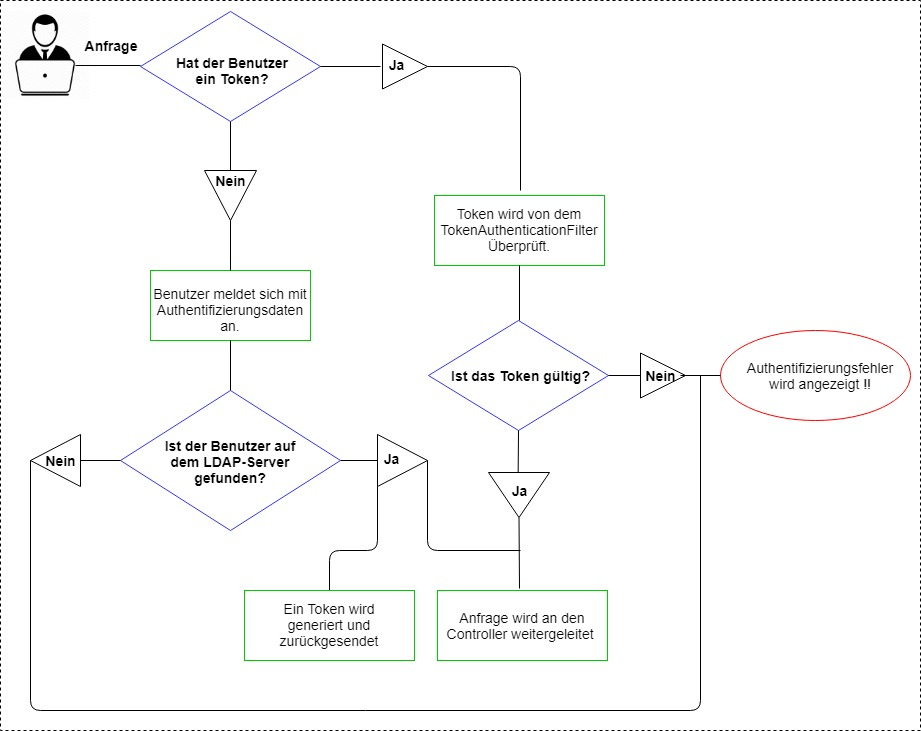
\includegraphics[width=15cm, height=15cm]{Ldap-Auth.jpg}
		\caption{Ldap-Auth } 
		\label{ Ldap-Auth } 
	\end{center}
\end{figure}
\newpage
\subsection{Erstellung eines neuen Aufgabenblatts (Admin)}
Wie oben erläutert, ist die Erstellung eines neuen Aufgabenblatts in der Tat eine Einrichtung eines neuen Testbereichs, an dem die Studenten ihre Aufgabenlösungsdateien testen können. Mit anderen Worten, das Erstellen eines neuen Aufgabenblatts hängt vom Erstellen eines neuen Git-Repository ab, das denselben Namen wie das Aufgabenblatt hat. Zum Beispiel (Aufgabenblatt-1) über die Gogs-Oberfläche, die dem Administrator zur Verfügung steht. In diesem Git-Gogs-Repository werden alle zum Testen erforderlichen Dateien gespeichert. Anschließend wird ein Jenkins Multibranch-Pipeline-Job erstellt, der auch denselben Namen wie das Aufgabenblatt hat.
\subsection{Schaffung von Jenkins Job (Admin)}
Für die Erstellung von Multibranch-Pipeline-Job, Jenkins bietet eine REST-API an, die viele Dienste bereitstellt, z. B. das Erstellen und Löschen von Job und viele andere Dinge. Um diese Jenkins-API zu verwenden, muss eine Maven-Abhängigkeit in pom.xml hinzugefügt werden.
\begin{lstlisting}[language=XML,caption=pom.xml - Jenkins-Api]
<dependency>
<groupId>com.offbytwo.jenkins</groupId>
<artifactId>jenkins-client</artifactId>
<version>0.3.7</version>
</dependency>
\end{lstlisting}
Zur Verdeutlichung wird erläutert, wie mit Jenkins-Api einen neuen Job erstellt werden kann. Um einen Job in Jenkins zu erstellen, müssen dem Job  ein Name und eine Reihe von Einstellungen nach Bedarf  zugewiesen werden.
\newline
Der Jobname wird als String  für die Jenkins-Api-Methode angegeben und die Einstellungen (Konfigurationen) werden jedoch als XML-Datei dargestellt.
\begin{lstlisting}[language=JAVA,caption=JenkinsServiceImp - createJob]
@Override
public void createJob(String jobName, String jobXml) throws JenkinsException {
try{
JenkinsServer jenkinsServer = new JenkinsServer(new URI(jenkinsUrl), jenkinsUser, jenkinsPassword);
jenkinsServer.createJob(jobName, jobXml, true);
}catch (Exception e){
throw new JenkinsException(e);
} 
}
\end{lstlisting}
Die Idee dabei ist, dass in diesem Fall jeder Jenkins-Job die gleichen Einstellungen wie die anderen hat. Unabhängig davon, für welches Aufgabenblatt der Job erstellt wurde. Daher ist es ausreichend, bei jeder Erstellung eines Jenkins-Jobs dieselbe Konfigurationsdatei (XML-Datei) zu verwenden. Natürlich mit einigen Änderungen, die behoben werden, wie die Git Repository URL. Zu diesem Zweck wird ein Java-XML-Parser eingesetzt. Es sind viele Java XML-Parser verfügbar. In diesem Fall wird der DOM-Parser benutzt. Der DOM-Parser lädt die XML-Datei in den Speicher und gibt dem Programmierer dann die Möglichkeit die XML-Datei Knoten für Knoten durchzulaufen, um sie zu analysieren. DOM-Parser eignet sich für kleine Dateien. Mit zunehmender Dateigröße verlangsamt sich die Leistung und der Arbeitsspeicher wird erhöht.
\begin{lstlisting}[language=JAVA,caption=modifyXmlFil]
public String modifyXmlFile(String jobname) throws ParserConfigurationException, SAXException, IOException {
DocumentBuilderFactory factory = DocumentBuilderFactory.newInstance();
try {
DocumentBuilder builder = factory.newDocumentBuilder();
File file = new File("config.xml");
Document doc = builder.parse(file);
Element element = doc.getDocumentElement();
NodeList nodes = element.getChildNodes();
NodeList  sources = nodes.item(19).getChildNodes();
Node  data =  sources.item(1);
Node  branchSource =  data.getChildNodes().item(1);
Node  source =  branchSource.getChildNodes().item(1);
NodeList sourceNodes = source.getChildNodes();
Node remote = sourceNodes.item(3);
remote.setTextContent("http://172.23.0.3:3000/swissi/"+jobname+".git");
DOMSource domSource = new DOMSource(doc);
StringWriter writer = new StringWriter();
StreamResult result = new StreamResult(writer);
TransformerFactory tf = TransformerFactory.newInstance();
Transformer transformer = tf.newTransformer();
transformer.transform(domSource, result);
return writer.toString();    
} catch (Exception ex) {
ex.printStackTrace();
return null;}}
\end{lstlisting} 
Was jetzt fehlt, um den neuen Testberich zu vervollständigen ist, das Hochladen der zum Testen notwendigen Dateien. Diese Dateien und ihre Rolle beim Abschließen des Testprozesses werden später ausführlich besprochen, aber jetzt geht es darum, wie sie hochgeladen und an die Remote-Testumgebung gesendet werden.

\subsection{Zum Testen notwendigen Dateien hochzuladen}
Nach dem Hochladen werden die Dateien in ihrem jeweiligen Git-Repository gespeichert. Um dies zu veranschaulichen, ist es wünschenswert, paar Git-Konzepte zu erwähnen.
\newline
Git hat zwei Repository-Typen: lokal und remote. Das lokales Repository wird aus einem Remote-Repository erstellt (Clone). Das Senden (Pushing) von Dateien und Code-Änderungen vom lokalen Repository bis zum Remote-Repository erfolgt in mehreren Schritten: 
\begin{itemize}
	\item Add: Dadurch werden neue oder aktualisierte Dateien in die „Stage“ oder den „Index“ kopiert.
	\item Commit: Dadurch werden die bereitgestellten Dateien in das lokale Repository kopiert.
	\item Push: Dadurch werden Ihre Dateien vom lokalen Repo auf das Remote-Repo kopiert (nur die Änderungen, die die Remote-Repos nicht haben).
\end{itemize}
\begin{figure}[h!]
	\begin{center}
		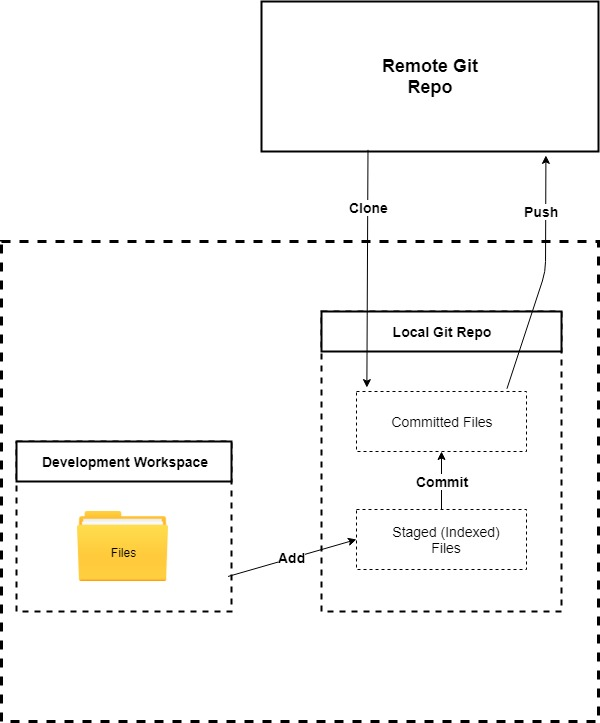
\includegraphics[width=12cm, height=8cm]{Git-Konzept.jpg}
		\caption{Git-Konzepte} 
		\label{ Git-Konzepte} 
	\end{center}
\end{figure}
\newpage
Nun wird erklärt, wie das oben Genannte Git-Konzepte in diesem Fall angewendet wird. 
\newline
Um Git aus einem Java-Programm zu verwenden, gibt es eine voll funktionsfähige Git-Bibliothek namens JGit. JGit ist eine relativ vollständige Implementierung von Git, die ursprünglich in Java geschrieben wurde und in der Java-Community weit verbreitet ist.
Es gibt verschiedene Möglichkeiten, ein Projekt mit JGit zu verbinden und Code dagegen zu schreiben. Am einfachsten ist wahrscheinlich die Verwendung von Maven - die Integration erfolgt durch Hinzufügen des folgenden Snippets zum <dependencies>Tag in der pom.xml-Datei:
\begin{lstlisting}[language=XML,caption=JGit-dependency ]
<dependency>
<groupId>org.eclipse.jgit</groupId>
<artifactId>org.eclipse.jgit</artifactId>
<version>3.5.0.201409260305-r</version>
</dependency>
\end{lstlisting} 
Angenommen, der Administrator hat ein Remote-Git-Repository für ein bestimmtes Aufgabenblatt erstellt. Aus diesem Remote-Repository wird durch Git.cloneRepository () ein lokales Repository gemacht.
\begin{lstlisting}[language=JAVA,caption=clone Repository ]
public static Git cloneRepo(String repositoryUrl, String gitLocalRepositoryPath, String tfsUser, String password) throws GitAPIException, IOException {
   Path path = Paths.get(gitLocalRepositoryPath);
  if (!Files.exists(path)) {
  CloneCommand cloneCommand = Git.cloneRepository().setURI(repositoryUrl).setDirectory(new File(gitLocalRepositoryPath));
  UsernamePasswordCredentialsProvider user = new UsernamePasswordCredentialsProvider(tfsUser, password);
  cloneCommand.setCredentialsProvider(user);
  Git repository = cloneCommand.call();
  return repository;
  }else{Git repository = Git.open(new File(gitLocalRepositoryPath));
   System.out.println("exist" + repository.toString());

  return repository;
}
}
\end{lstlisting} 
Dieses lokale Repository wird sich in einem BackEnd-Ordner namens 'aufgabenblaetter' befindet. Die zum Ausführen des Tests erforderlichen Dateien werden nach dem Upload in diesem BackEnd-Ordner in seinem eigenen lokalen Repository gespeichert. Wenn beispielsweise Dateien zum Test von Aufgabenblatt-1 hochgeladen werden, werden sie unter 'aufgabenblaetter/Aufgabenblatt-1' gespeichert.
\newline
Jetzt erfolgt der Versand (Push) von Dateien vom lokalen Repository zum Remote-Repository. Wie bereits erwähnt, besteht dieser Prozess aus drei Schritten. Zunächst werden die Änderungen mit der von der Git-Bibliothek bereitgestellten add-Methode zum Staging-Bereich hinzugefügt.
\begin{lstlisting}[language=JAVA,caption=Add File To Index ]
public static boolean addFileToIndex(Git repository) throws IOException, GitAPIException {
try {
repository.add().addFilepattern(".").call();
return true;
} catch (Exception e) {
System.out.println(e.getMessage());
}
return false;
}
\end{lstlisting} 
Zweitens wird ein neues Commit mit dem aktuellen Inhalt des Index erstellt.
\begin{lstlisting}[language=JAVA,caption=commit Changes ]
	public static boolean commitChanges(Git repository, String commitMessage) throws GitAPIException, IOException {
repository.commit()
.setAll(true)
.setMessage("Commit changes to all files")
.call();

System.out.println("Committed all changes to repository at ");
return true;
}
\end{lstlisting} 
Drittens werden Commits vom lokalen Repository an das Remote-Repository übertragen.
\begin{lstlisting}[language=JAVA,caption=Push Changes ]
public static boolean pushChanges(Git repository) throws GitAPIException, URISyntaxException, IOException {
try
{
PushCommand pushCommand = repository.push();
pushCommand.setCredentialsProvider(new UsernamePasswordCredentialsProvider("swissi", "Mh123456"));
pushCommand.call();
return true;
}
catch (GitAPIException e)
{
throw new RuntimeException(e);
}
}
\end{lstlisting} 

 \newpage
\subsection{Die zum Ausführen des Tests erforderlichen Dateien}
Jedes Git-Repository, das die Quellcodeverwaltung für ein bestimmtes Aufgabenblatt in der Remote-Testumgebung darstellt, hat die folgende Form und als Beispiel den folgenden Inhalt.
\newline
\dirtree{%
	.1 Aufgabenblatt-N.
	.2 makefile.
	.2 Jenkinsfile.
	.2 src.
	.3 ulam.c .
	.2 test.
	.3 ppr-tb-test-ulam.c.
}

Jedes Repository, unabhängig davon, welchem Aufgabenblatt es zugewiesen ist, enthält immer ein Makefile, ein Jenkinsfile, einen src-Ordner und einen test-Ordner.
\begin{itemize}
    \item \textbf{Src-Ordner: } Dies ist der unter-Repository-Ordner, in den der Student seine Aufgabenblattlösung hochladen wird. Dieser Vorgang wird nachstehend ausführlich erörtert.
	\item \textbf{Test-Ordner: } Hier wird die Datei mit den Testfällen vom Administrator hochgeladen.
	\item \textbf{Makefile: }  Wie bereits erwähnt, gibt es eine vom Administrator hochgeladene Testdatei und eine andere vom Studenten hochgeladene Lösungsdatei. Dies bedeutet, dass mehrere Quelldateien kompiliert werden müssen, um das Projekt zu bauen und ein Testergebnis zu erhalten. Um diesen Prozess zu erleichtern und solches Hindernis zu überwinden wird in diesem Fall ein Makefile benutzt.
	\newline
	Ein Makefile wird mit dem UNIX-Dienstprogramm 'make' verwendet, um zu bestimmen, welche Teile eines Programms kompiliert werden sollen. Ein Makefile ist im Grunde ein Skript, mit dem das Dienstprogramm make die geeigneten Programmdateien auswählt, die kompiliert und miteinander verknüpft werden sollen. Das Dienstprogramm make protokolliert die letzten Aktualisierungen von Dateien, sodass nur die Dateien aktualisiert werden, die Änderungen enthalten. Es müssen jedoch auch alle Dateien kompiliert werden, die von den aktualisierten Dateien abhängig sind, was sehr zeitaufwändig sein kann. Mit Hilfe von makefile automatisiert das Dienstprogramm make diese Kompilierung, um sicherzustellen, dass alle aktualisierten Dateien - und nur diese - kompiliert werden und dass die neuesten Versionen der Dateien mit dem Hauptprogramm verknüpft sind.
	\newline
	Ein Makefile enthält drei Arten von Informationen für das make-Programm: ein Ziel oder auch target genannt wird, das normalerweise der Name einer Datei, die von einem Programm generiert wird. Beispiele ausführbare Dateien oder Objektdateien. Es enthält auch Abhängigkeiten und Regeln (Befehle), die angeben, wie das Ziel aus den Quellen erstellt werden soll. 
	 
	\item \textbf{Jenkinsfile: } Ist eine Textdatei, die die Definition einer Jenkins-Pipeline enthält und in die Quellcodeverwaltung eingecheckt wird. Die Rolle dieser Datei wird nachfolgend erläutert.
	\end{itemize}
Bevor zu den folgenden Abschnitten übergangen wird, wird erläutert,wie der Student seine Lösungsdatei hochladen kann.
\subsection{Student-Lösungsdatei hochladen}
Der Student lädt die zu testende Datei über die Frontend-Seite. Er wählt die Datei aus und drückt dann die Upload-Button. Das Backend erhält also eine Anfrage zum Hochladen von Dateien. Um diese Aufgabe auszuführen, muss das BackEnd die folgenden Schritte ausführen: Angenommen, der Benutzer möchte seine Aufgabenblatt-1-Lösung zum ersten Mal testen. Anschließend wird aus dem lokalen Git-Repository von Aufgabenblatt-1 ein Branch mit dem Benutzernamen als Namen erstellt.

\begin{lstlisting}[language=JAVA,caption= createBranch ]
public static void createBranch(Git repository, String branchName) throws IOException, GitAPIException {
String current = currentBranch(repository);
if (Objects.equals(current, branchName)) {
return;
}
System.out.println("Checking out branch: " + branchName);
// lets check if the branch exists
CheckoutCommand command = repository.checkout().setName(branchName);
boolean exists = localBranchExists(repository, branchName);
if (!exists) {
command = command.setCreateBranch(true).setForce(true).
setUpstreamMode(CreateBranchCommand.SetupUpstreamMode.TRACK);

}
Ref ref = command.call();
if (LOG.isDebugEnabled()) {
LOG.debug("Checked out branch " + branchName + " with results " + ref.getName());
}
configureBranch(repository, branchName);

}
\end{lstlisting} 

Dann wird Die Datei durch Ausführen der Methoden Jgit-add und -commit an den angegebenen Branch gesendet. Der Benutzer hat nun die Möglichkeit, entweder den Test abzubrechen, was bedeutet, dass die hochgeladene Datei gelöscht wird, oder fortzufahren hat und den Test-Button zu drücken. Angenommen, der Benutzer den Test abgeschlossen und die Test-Button gedrückt. Dann wird der Student-Branch durch eine Jgit-Push-Methode an das Remote-Repository übertragen. Zur weiteren Verdeutlichung wird eine grafische Darstellung angezeigt, die diesen Vorgang erläutert.
\begin{figure}[h!]
	\begin{center}
		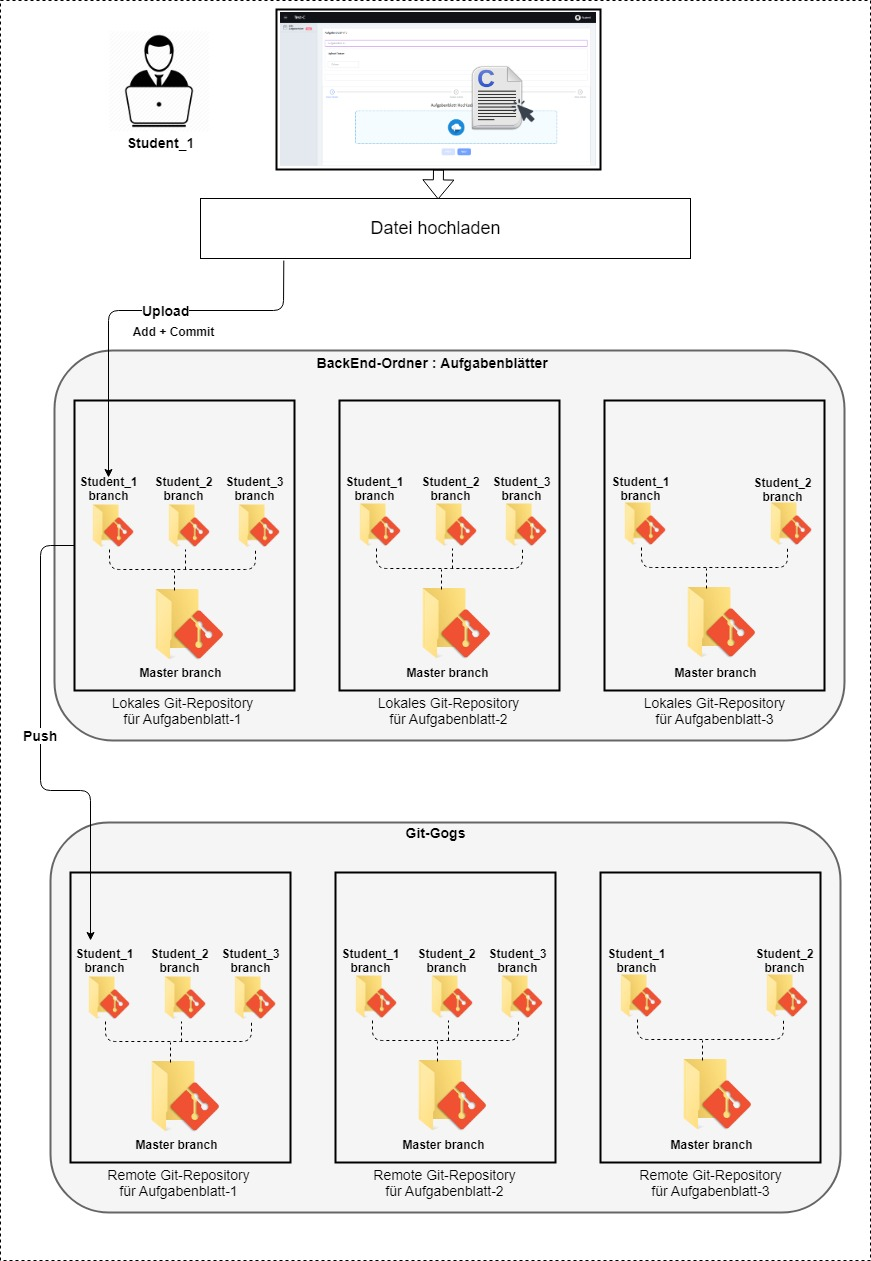
\includegraphics[width=14cm, height=15cm]{Loesungupload.jpg}
		\caption{Hochladen von Lösungsdatei} 
		\label{ Hochladen von Lösungsdatei } 
	\end{center}
\end{figure}
\newpage
Für jedes Aufgabenblatt wird ein lokales und ein remote Git-Repository erstellt. Für jeden Student wird aus jedem Aufgabenblatt-Repository ein Branch erzeugt. 
\newline
Es wird beispielsweise davon ausgegangen, dass der Administrator drei Aufgabenblätter hinzufügt. Das heißt, es werden drei Git-Repositorys erstellt, jedes von denen ein Aufgabenblatt darstellt. Drei Studenten möchten ihre Lösungen testen. Zwei von ihnen haben die drei Übungsblätter gelöst und einer hat nur das erste und das zweite Aufgabenblatt gelöst. Anschließend werden aus den für die Aufgabenblätter 1 und 2 erzeugten Git-Repositorys drei Branchs erstellt. Weil die drei Studenten die ersten beiden Übungsblätter gelöst und getestet haben. Aus dem dritten Repositroy werden jedoch nur zwei Branchs erzeugt, da nur zwei Studenten ihre Aufgabenblatt-3-Lösung getestet haben.
\newline
Nun wird besprochen, wie nach Erhalt der Lösungsdatei der Test Prossez automatisch gestartet und das Ergebnis dem Student angezeigt wird.
\subsection{Test Starten (jenkins Job Build)}
Wie bereits erwähnt, wird für jedes Repository automatisch ein Jenkins-Multibranch-Pipeline-Job generiert. Ein Multibranch-Pipeline-Job durchsucht einfach das Quellcode-Repository und erstellt automatisch einen Pipeline-Job für jedes Branch, das eine Jenkinsfile-Datei enthält. 
\newline
Eine Jenkinsfile-Datei ist eine Textdatei, die die Pipeline als Skript enthält, der den gesamten Job-Workflow festschreibt. Daher lädt der Administrator diese Datei bei jeder Erstellung eines neuen Aufgabenblatts hoch. Dieser Vorgang ist in der folgenden Grafik dargestellt.
\begin{figure}[h!]
	\begin{center}
		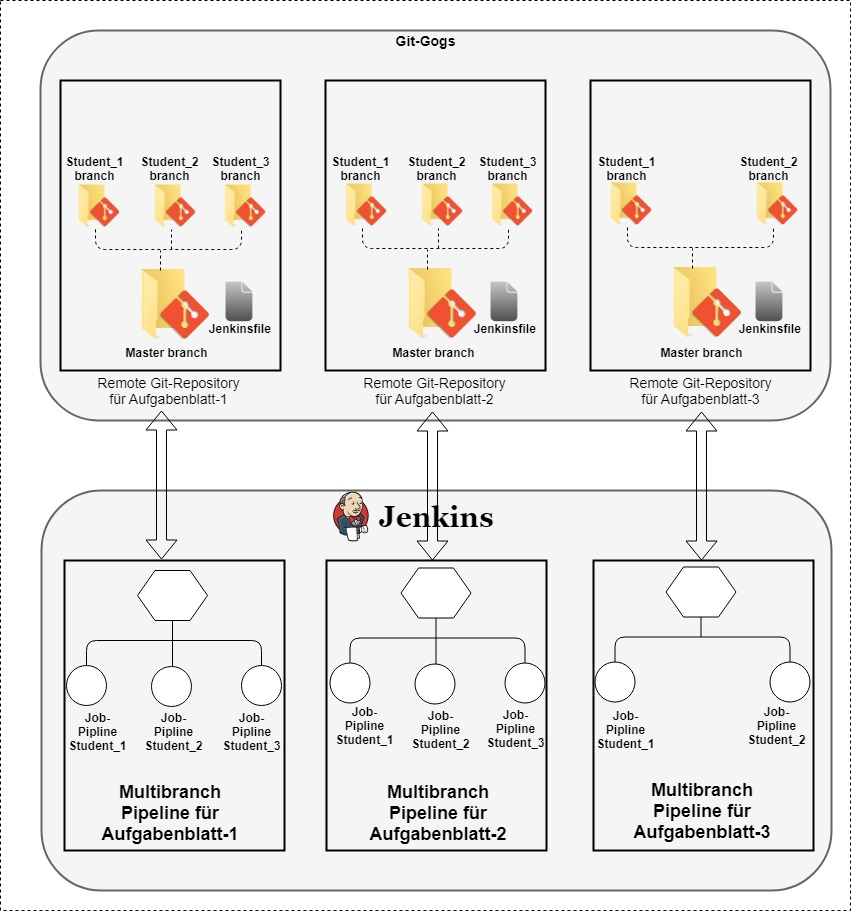
\includegraphics[width=13cm, height=13cm]{GogsJenkins.jpg}
		\caption{Multibranch Pipeline Job} 
		\label{ Multibranch Pipeline Job } 
	\end{center}
\end{figure}
\newpage
In diesem Fall besteht die Job-Pipeline nur aus einer Phase (stage), in der das Makefile ausgeführt werden sollte, um den Testprozess zu starten. Genau das, was in der Jenkinsfile-Datei steht.
\begin{lstlisting}[language=JAVA,caption=Jenkinsfile (Job-Pipeline-Skript) ]
pipeline{
agent any
stages {   
   stage ('Test with make file') {
       steps {
         sh 'make'
             }
       }
       }
      }
\end{lstlisting} 
'make' ist der Befehl zum Ausführen von makefile.
\newline
Jetzt werden sich die Ideen neu gruppieren und klar aufbauen. Der 'Student-1' hat die zu testende Datei hochgeladen. Zum Beispiel die Lösung von Übungsblatt-1. Wenn er seine Aufgabenblattlösung zum ersten Mal testet. Ein Branch namens 'Student-1' wird vom Aufgabenblatt-1-Repository erzeugt .Dann wird die Datei an diesem Branch übergeben.Wenn dies nicht der Fall ist und der Student diese Übungsblattlösung bereits getestet hat, ist eventuell ein Branch vorhanden, das einfach verwendet wird. Wenn der Benutzer die Testschaltfläche gedrückt hat, wird Student-1-Branch nach Remote verschoben, wenn es zum ersten Mal erstellt wurde. Wird jedoch bereits eine mit demselben Namen erzeugt, werden nur die Änderungen übertragen. Danach sendet das BackEnd eine Job-Build Anfrage mit dem Job-Namen 'Aufgabenblatt-1' an den Jenkins-Server. 
\begin{lstlisting}[language=JAVA,caption=Job-Build Anfrage ]
	public int buildJob(String jobName) throws JenkinsException {
int buildNumber = 0;
try{
JenkinsServer jenkinsServer = new JenkinsServer(new URI(jenkinsUrl), jenkinsUser, jenkinsPassword);
Map<String, Job> jobs = jenkinsServer.getJobs();
JobWithDetails job = jobs.get(jobName).details();
buildNumber = job.getNextBuildNumber();
job.build(true);
}catch (Exception e){
throw new JenkinsException(e);
}
return buildNumber;
}
\end{lstlisting} 
Wichtig: Wenn eine Lösungsdatei hochgeladen wurde, wird der Benutzer aufgefordert, den Namen des Aufgabenblatts einzugeben, zu dem die Lösungsdatei gehört. Somit kann das Backend unterscheiden, welches Git-Repository und welcher Jenkins-Job verwendet werden soll. Das beste Beispiel, um dies zu veranschaulichen, ist diese Build-Job-Methode (Listing 4.11), die den Namen des auszuführenden Jobs (JobName) als Parameter verwendet. In diesem Fall lautet der Jobname 'Aufgabenblatt-1', der von Student beim Hochladen der Datei angegeben wird.
\newline
Wenn Jenkins Server eine Build-Anfrage für einen Multibranch-Pipeline-Job erhält, sucht er nach neuen Branches im 'Git-Repository' oder nach Änderungen in alten Branches. Dann wird für jeden neuen Zweig (Branch) oder Zweig, der die Änderungen enthält, ein Build gebaut.
\newline
In diesem Fall ist das Erstellen eines Jenkins-Builds in der Tat eine Kompilierung des Makefiles, um den Testprozess abzuschließen.
\newline
Beim Kompilieren des Makefiles werden die Testdateien und die zu testenden Dateien vom GCC-Compiler in Objektdateien bzw. Programmmodule umgewandelt. Dann wird der Verknüpfungsschritt ausgeführt und eine Binärdatei (executable) erzeugt. In diesem Fall ist die Binärdatei das Testergebnis. Diesen Vorgang wird in der nächsten Grafik veranschaulicht.
\newpage
\begin{figure}[h!]
	\begin{center}
		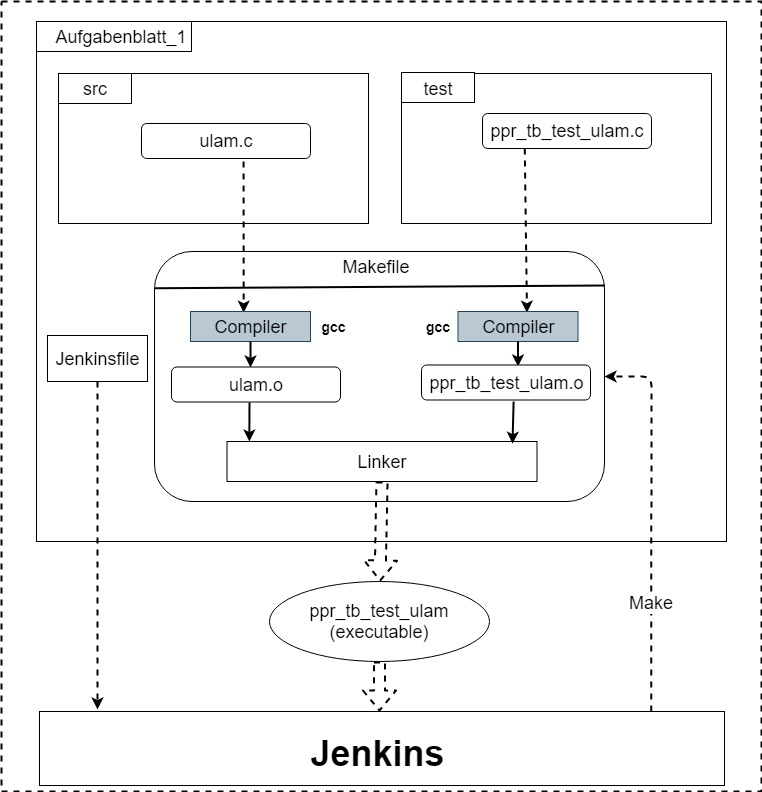
\includegraphics[width=15cm, height=17cm]{Makefile.jpg}
		\caption{Kompilieren des Programms} 
		\label{Kompilieren des Programms} 
	\end{center}
\end{figure}

Nach Abschluss des Build-Prozesses wird das Testergebnis im Build-Verlauf des Jenkins-Servers gespeichert. Was jetzt fehlt, ist dem Benutzer das Testergebnis anzuzeigen. Darüber wird im nächsten Absatz besprochen.
\newpage
\subsection{Testergebnis anzeigen}
 Der Multibranch-Pipeline-Job speichert einen Build-Verlauf für jeden Zweig (Branch). Der Buildverlauf enthält Builddetails. Aus Build-Details kann ConsoleOutputText abgerufen werden. In diesem Fall enthält dieser 'ConsoleOutputText' das Testergebnis.
 \begin{lstlisting}[language=JAVA,caption=Testergebnis Anfrage ]
public StringBuilder jenkinsgetjobCosole(String jobName, String branchName ) throws JenkinsException {
String buildLog = "";
int i = 0;
StringBuilder buildLogBuilder = null;
try {
JenkinsServer jenkinsServer = new JenkinsServer(new URI(jenkinsUrl), jenkinsUser, jenkinsPassword);
Map<String, Job> jobs = jenkinsServer.getJobs();
JobWithDetails job = jobs.get(jobName).details();
Optional<FolderJob> folderJob = jenkinsServer.getFolderJob(job);
Map<String, Job> branchs = jenkinsServer.getJobs(folderJob.get());
String currentUser = SecurityContextHolder.getContext().getAuthentication().getName();
JobWithDetails branch = branchs.get(currentUser).details();
Build build = branch.getLastBuild();
if (build != null) {
BuildWithDetails buildWithDetails = build.details();
buildLog = buildWithDetails.getConsoleOutputText();
Reader inputString = new StringReader(buildLog);
BufferedReader reader = new BufferedReader(inputString);
buildLogBuilder = new StringBuilder();  
/*Hier wird der 'buildLogBuilder' bearbeitet, um ihn dem Benutzer klar zu zeigen.*/
return buildLogBuilder;
} catch (Exception e) {
throw new JenkinsException(e);
}}
 \end{lstlisting}
 \newpage
 Zunächst werden alle Jobs abgerufen, die sich auf dem Jenkins-Server befinden. Innerhalb dieser Jobs wird der gewünschte Job identifiziert, zum Beispiel 'Aufgabenblatt-1'. Dann werden alle UnterJobs-Zweige, die in diesem Job sind, gebracht und daraus der gewünschte UnterJobs-Zweig festgestellt. Von diesem  UnterJobs-Zweig wird das letzte Build-Detail abgerufen. Schließlich wird das Testergebnis (ConsoleOutputText) aus dieses Build-Detail erhalten. Die folgende Abbildung zeigt diesen Vorgang grafisch.
 \begin{figure}[h!]
 	\begin{center}
 		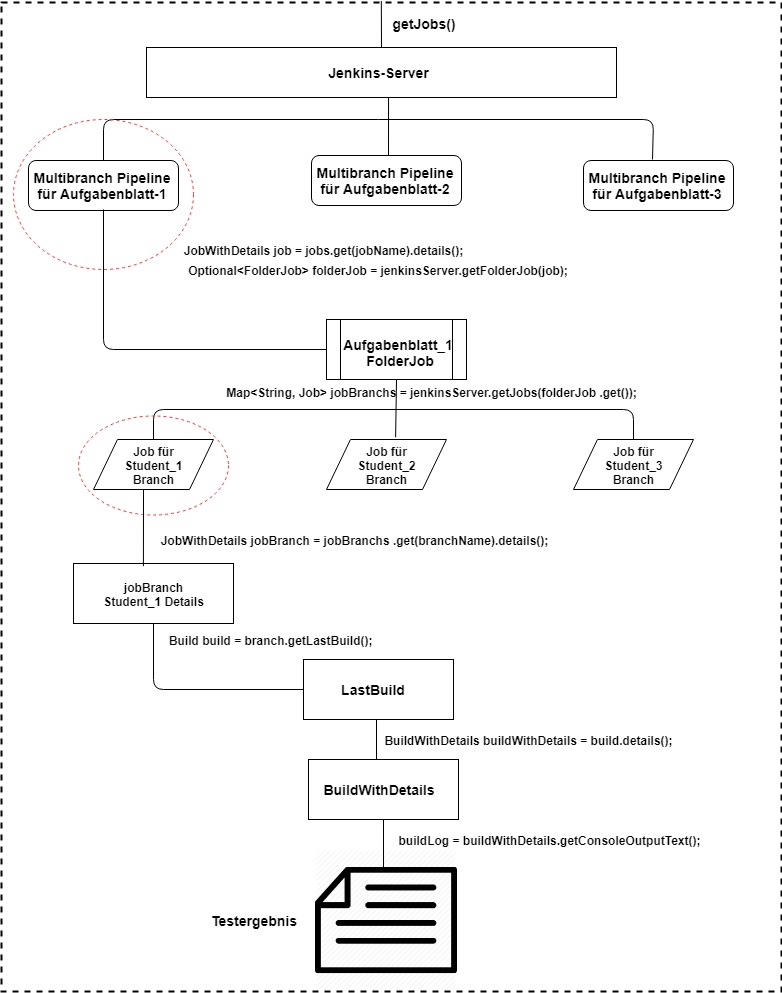
\includegraphics[width=14cm, height=16cm]{TestergebnisOutput.jpg}
 		\caption{jenkinsgetjobCosole} 
 		\label{jenkinsgetjobCosole} 
 	\end{center}
 \end{figure}

Das Testergebnis wird dann an das Front-End gesendet, um es dem Benutzer anzuzeigen.
\newpage
\section{Installationsanleitung}
Im Abschnitt 'Architektur' wurde bereits erwähnt, dass die Komponenten des Projekts in Docker bereitgestellt werden. Dies wird in diesem Abschnitt mit der Erklärung der für den Installationsprozess erforderlichen Einstellungen erläutert.
\subsection{Projektbereitstellung (deployment)}
Docker ist eine container-basierte Technologie und Container sind nur der Benutzerbereich des Betriebssystems. Auf der niedrigen Ebene ist ein Container nur eine Reihe von Prozessen, die vom Rest des Systems isoliert sind und von einem separaten Image ausgeführt werden, das alle zur Unterstützung der Prozesse erforderlichen Dateien enthält. In Docker teilen sich die ausgeführten Container den Kernel des Host-Betriebssystems. Docker ist ein Open-Source-Projekt, das auf Linux-Containern basiert. Es verwendet Linux-Kernel-Funktionen wie Namespaces und Kontrollgruppen, um Container auf einem Betriebssystem zu erstellen. Docker fügt die Software einer Anwendung in eine unsichtbare Box ein, in der alles enthalten ist, was zum Ausführen erforderlich ist, z. B. Betriebssystem, Anwendungscode, Laufzeit, Systemtools und Bibliotheken usw.
\newline
Um zu verstehen, wie Docker am besten eingesetzt wird, ist es hilfreich, sich einen groben Überblick darüber zu verschaffen, wie die Docker-Plattform aufgebaut ist.
\begin{figure}[h!]
	\begin{center}
		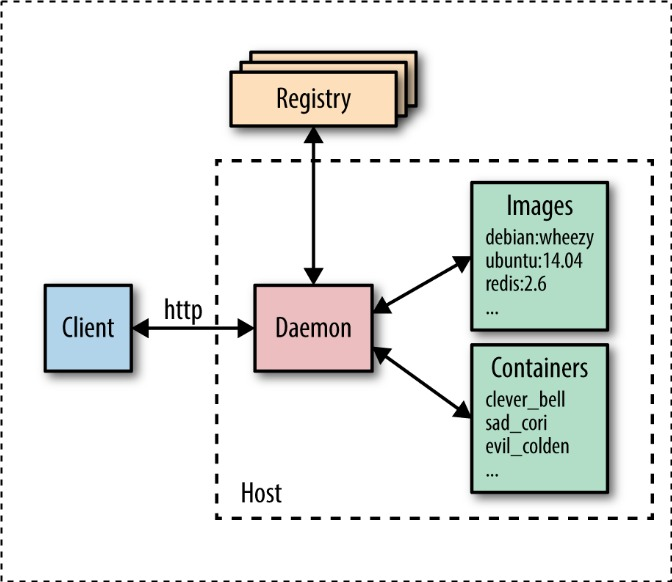
\includegraphics[width=13cm, height=7cm]{Docker-components.jpg}
		\caption{Docker-Komponenten} 
		\label{Docker-Komponenten} 
	\end{center}
\end{figure}
\begin{itemize}
	\item \textbf{Docker-Daemon: }der Docker-Daemon ist für das Erstellen, Ausführen und Überwachen von Containern, Netzwerke und Volumes sowie für das Erstellen und Speichern von Images zuständig.
	\item \textbf{Docker-Client: }Dies ist das Command Line Interface (CLI)-Tool, das zur Konfiguration und Interaktion mit Docker verwendet wird. Zum Beispiel wenn Entwickler oder Benutzer Befehle wie Docker Run verwenden, sendet der Client diese Befehle an den Docker-Daemon, der sie ausführt.
	\item \textbf{Images: }Sind abstrakte Container, die bestimmte Prozesse am Laufen halten. Diese Prozesse aus der Dockerfile abgelesen und als Read-Only Datei-Systemen angelegt.
	\item \textbf{Docker file: }Ein Dockerfile ist einfach eine Textdatei mit einer Reihe von Anweisungen (instructions), die genutzt werden können, um ein Docker-Image zu erzeugen.
	\item \textbf{Containers: }Container ist die ausgeführte Instanz eines Images. Mit einen Read-Write Dateisystem, die Container spezifische Infos enthält (Ip Adresse , Ports, etc).
	\item \textbf{Networking: }Damit Docker-Container über den Host-Computer miteinander und mit der Außenwelt kommunizieren können, wird eine Netzwerkschicht (Docker Networking) eingesetzt. Docker unterstützt verschiedene Arten von Netzwerken, die jeweils für bestimmte Anwendungsfälle geeignet sind: Bridge mode, Host mode, Container mode, und No networking.
	\item \textbf{Docker Registries: }Dies ist die Distributionskomponente von Docker oder wird als zentrales Repository für Docker-Images bezeichnet, in dem Docker-Images gespeichert sind. Docker Hub und Docker Cloud sind öffentliche Registrierungen, die von jedem Benutzer verwendet werden können. 
\end{itemize}
Nun wird erläutert, wie Docker in diesem Fall zum Bereitstellen der Anwendung verwendet wird. Die Anwendung 'Test-C-Plattform' wird in sechs Containern bereitgestellt. Zwei Container für das Front-End (AdminPortal-Container / Student Portal-Container), ein Container für das Back-End (Test C-Back-End-Container) und drei Container für die Remote-Testumgebung (Jenkins-Container / Gogs-Container / Postgresql-Container).
\newline
Wie bereits gesagt, ist ein Container die ausgeführte Instanz eines Images. Hier stellt sich die Frage, wie ein Image erstellt wird ?
\newline
In diesem Fall werden zwei verschiedene Typen von Images verwendet. Gebrauchsfertige Images, die in einem öffentlichen Repository wie Docker-Hub gespeichert sind, und mit Hilfe von Dockerfile selbst erstellte Images.
\newline
Die folgende Abbildung zeigt den Bereitstellungsprozess im Detail.
\newpage
\begin{figure}[h!]
	\begin{center}
		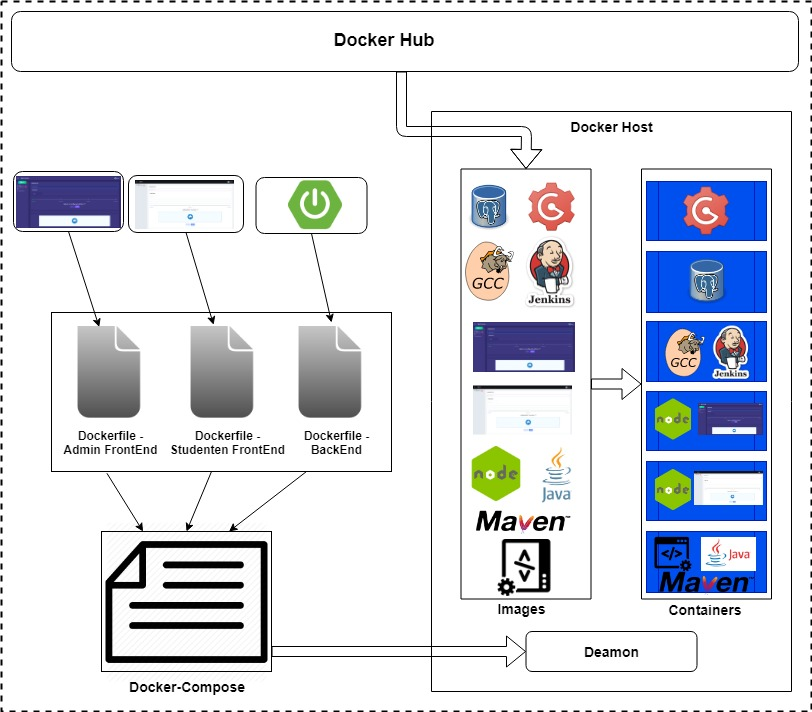
\includegraphics[width=16cm, height=18cm]{Application-deployment.jpg}
		\caption{Bereitstellungsprozess} 
		\label{Bereitstellungsprozess} 
	\end{center}
\end{figure}
\newpage
Dockerfile-Admin-FrontEnd und Dockerfile-Student-FrontEnd sind zuständig für die Erstellung von der beiden Angular Applications Images (AdminProtal und StudentenPortal).
\begin{lstlisting}[language=JAVA,caption=Dockerfile für Angular Application]
FROM node:lts-alpine as build-step
WORKDIR /app
COPY package.json ./
COPY . .
RUN npm install --save-dev node-sass
EXPOSE 4200
CMD npm run start
\end{lstlisting}
Die FROM-Anweisung legt fest, welches Basisimage von Docker-Hub zu verwenden ist,  wie in diesem Fall 'node'. RUN-Anweisunggen geben einen Schell-Befehl an, der im Image ausgeführt werden soll. COPY-Anweisunggen kopieren Dateien, die für die Umsetzung eines Images benötigen. CMD-Anweisung enthält CMD-Befehl, der nur ausgeführt wird, wenn ein Container ausgeführt wird.
\newline
Dockerfile-BackEnd ist für Erzeugung von BackEndTest-C Image verantwortlich.
\begin{lstlisting}[language=JAVA,caption=Dockerfile für BackEnd]
FROM maven:3-jdk-8-alpine
VOLUME /tmp
COPY ./target/backend-Test-C-1.5.8.RELEASE.jar /
RUN ls -l
CMD ["mvn","spring-boot:run"]
\end{lstlisting}
Das Basisimage hier ist maven:3-jdk-8-alpine. Das Jar Datei wird kopiert und durch Maven und Jdk ausgeführt.
\newline
Zum Definieren und Ausführen von Docker-Anwendungen mit mehreren Containern, wird Docker Compose verwendet.  Mit Compose wird eine YAML-Datei (docker-compose.yml) eingesetzt, um die Dienste (services) von der Anwendung zu konfigurieren, wobei jeder Dienst (service) einen Container mit der zum Erstellen erforderlichen Konfiguration darstellt.
\newpage
\begin{lstlisting}[language=JAVA,caption= Docker Compose]
version: '2'
services:
app:
image: gogs/gogs:latest
volumes:
- /tmp/gogs-data:/data
ports:
- "3000:3000"
links:
- postgres:postgres
postgres:
image: postgres:alpine
volumes:
- /tmp/gogs-postgres:/var/lib/postgresql/data
environment:
- POSTGRES_USER=postgres
- POSTGRES_PASSWORD=password123
- POSTGRES_DB=gogs
jenkins:
build:
context: .
dockerfile: ../jenkins-Dockerfile/Dockerfile
ports:
- "50000:50000"
- "8080:8080"
volumes:
- /var/jenkins_home  
image: jenkins/jenkins
adminPortal:
build:
context: .
dockerfile: ../test-C-Admin-Portal/Dockerfile
ports:
- "50001:50001"
- "4200:4200" 
image: adminportal  
studentenPortal:
build:
context: .
dockerfile: ../test-C-Studenten-Portal/Dockerfile
ports:
- "50003:50003"
- "8886:8886" 
image: studentenporstltest  
backendtestc:
build:
context: .
dockerfile: ../backend-Test-C/Dockerfile
ports:
- "50004:50004"
- "8088:8088" 
image: backend-test-c     
\end{lstlisting}
Für die ersten drei Dienste werden Docker Hub-Images gerippt und als Container an drei verschiedenen Ports ausgeführt. Für die anderen drei Dienste werden Dockerfiles aufgerufen, um zuerst die Images zu erstellen und dann jedes Image als Container auszuführen.
\newline
Standardmäßig richtet Compose ein einzelnes Netzwerk für die App ein. Jeder Container für einen Dienst tritt dem Standardnetzwerk bei und ist sowohl für andere Container in diesem Netzwerk erreichbar als unter einem Hostnamen erkennbar, der mit dem Containernamen identisch ist. 
\newline
Dazu muss Docker-Compose-file ausgeführt werden. Um eine Docker-Compose-Datei auszuführen, soll durch Docker-CLI (Command-line interface) das Command 'docker-compose up' an Docker-Deamon gesendet werden.
\newline
Nachdem der Daemon den Befehl erhalten hat, werden die Container ausgeführt und über ein Netzwerk miteinander kommuniziert.
\newpage
\begin{figure}[h!]
	\begin{center}
		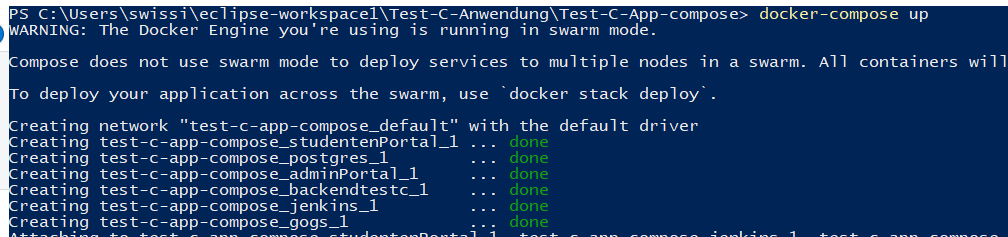
\includegraphics[width=17cm, height=5cm]{composeUp.PNG}
		\caption{docker-compose up} 
		\label{docker-compose up} 
	\end{center}
\end{figure}

Um zu überprüfen, ob das Netzwerk bereits erstellt wurde, kann der Befehl 'docker network ls' getippt werden.
\newline
\begin{figure}[h!]
	\begin{center}
		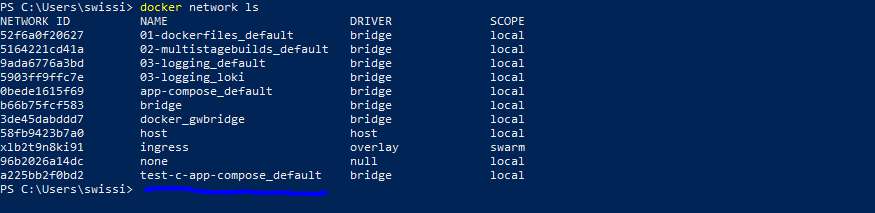
\includegraphics[width=17cm, height=5cm]{docker-network-ls.PNG}
		\caption{docker network ls} 
		\label{docker network ls} 
	\end{center}
\end{figure}
\newline
Mit dem Befehl 'docker network inspect <Name des Netzwerks>' wird überprüft, ob sich alle Container des Projekts bereits im Netzwerk befinden.
\newpage
\begin{figure}[h!]
	\begin{center}
		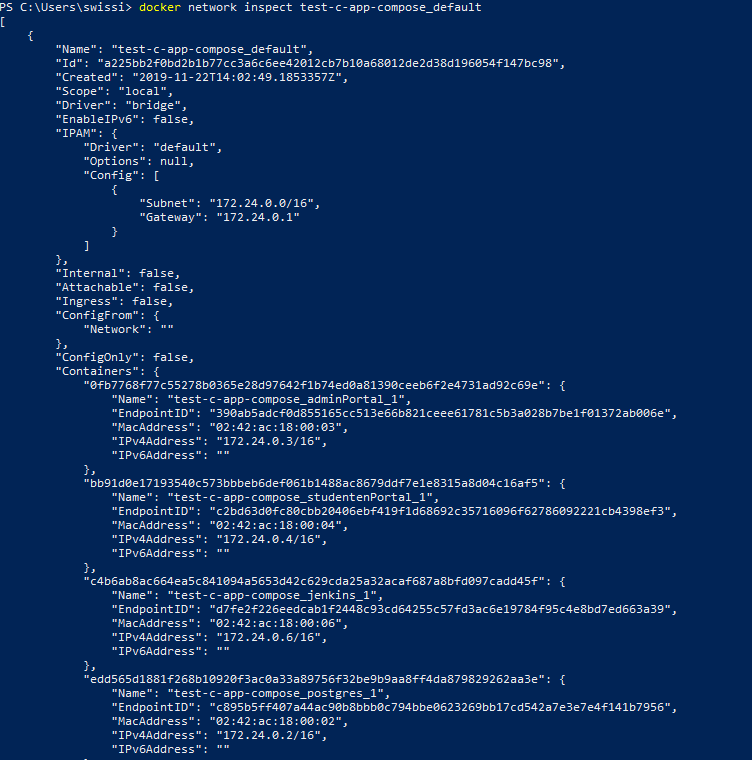
\includegraphics[width=14cm, height=14cm]{network-inspect.PNG}
		\caption{docker network inspect} 
		\label{docker network inspect} 
	\end{center}
\end{figure}
\subsection{Einstellungen}
\subsubsection{Konfigurieren von Gogs mit dem Web Installer}
Öffnen Sie https://example.com:3000 in Ihrem Browser. Sie werden zur Installationsseite weitergeleitet:
\begin{figure}[h!]
	\begin{center}
		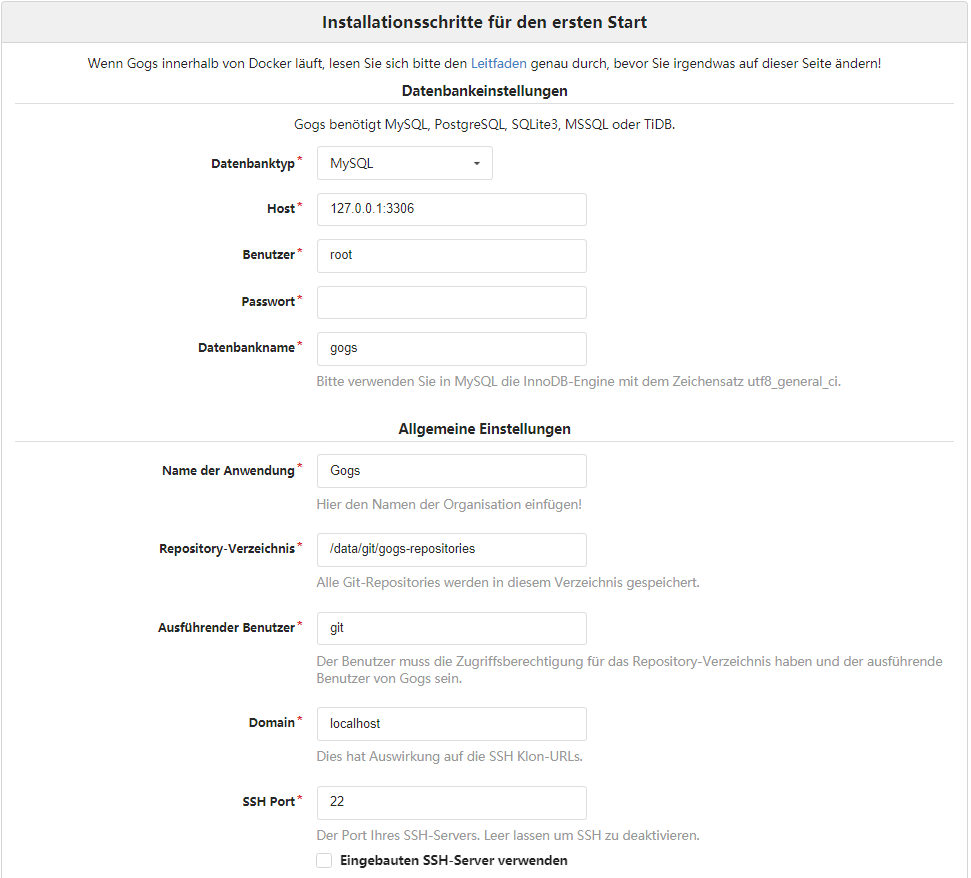
\includegraphics[width=15cm, height=17cm]{gogsWebInstaller.PNG}
		\caption{Gogs-Installationsseite} 
		\label{Gogs-Installationsseite} 
	\end{center}
\end{figure}
\newpage
Ändern Sie die Datenbankeinstellungen so, dass sie mit der zuvor erstellten PostgreSQL-Datenbank übereinstimmen:
\begin{itemize}
	\item \textbf{Datenbanktyp: }= PostgreSQL
	\item \textbf{Host: }= test-c-app-compose_postgres_1:5432
	\item \textbf{Benutzer: }= postgres
	\item \textbf{Passwort: }= password123
	\item \textbf{Datenbankname: }= gogs
\end{itemize}
Danach wird die Anmeldeseite angezeigt:
\begin{figure}[h!]
	\begin{center}
		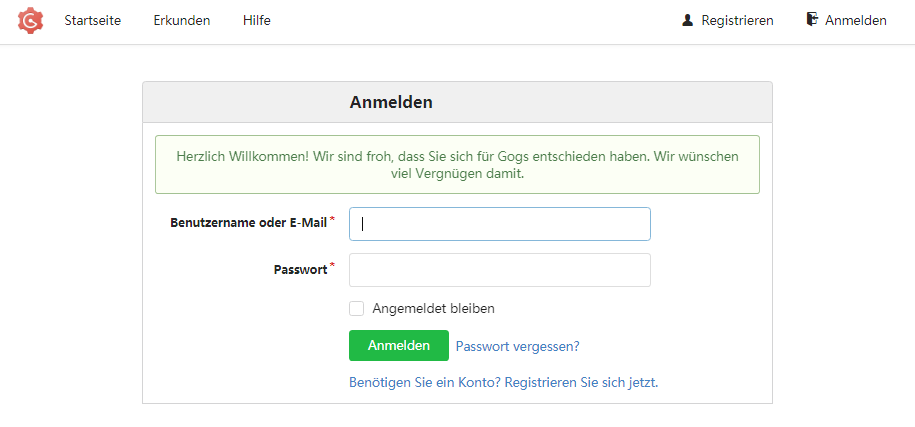
\includegraphics[width=17cm, height=8cm]{anmeldeseite.PNG}
		\caption{Gogs-Anmeldeseite} 
		\label{Anmeldeseite} 
	\end{center}
\end{figure}
\newline
Sie benötigen jetzt ein Gogs-Konto zu erstellen.
\begin{figure}[h!]
	\begin{center}
		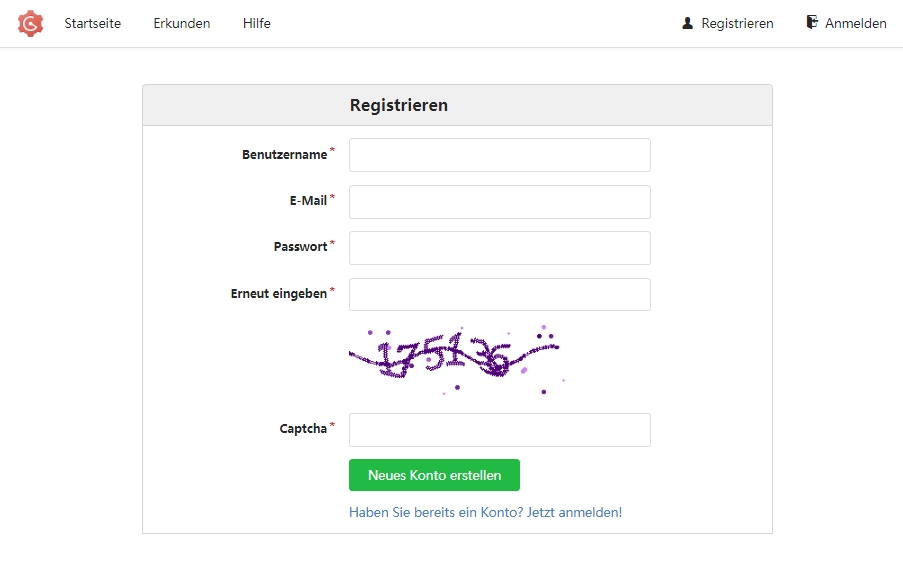
\includegraphics[width=17cm, height=8cm]{gogs-registrieren-seite.PNG}
		\caption{Gogs Registrieren Seite} 
		\label{Gogs Registrieren Seite} 
	\end{center}
\end{figure}
\subsubsection{Konfigurieren von Jenkins}
Wenn Sie zum ersten Mal auf eine neue Jenkins-Instanz zugreifen, werden Sie aufgefordert, diese mit einem automatisch generierten Kennwort zu entsperren.
Navigieren Sie zu https://example.com:8080, und warten Sie, bis die Seite Jenkins entsperren angezeigt wird.
\begin{figure}[h!]
	\begin{center}
		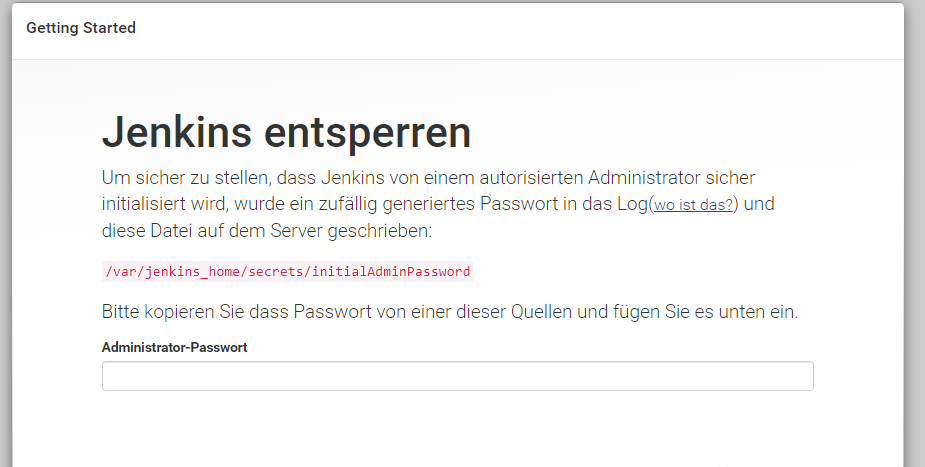
\includegraphics[width=17cm, height=7cm]{Jenkins-entsperren-seite.PNG}
		\caption{Jenkins entsperren Seite} 
		\label{Jenkins entsperren Seite} 
	\end{center}
\end{figure}
\newpage
Das automatisch generierte Passwort finden Sie in den Protokollen von Jenkins-Container. Sie können dies mit dem folgenden Befehl tun: 'docker logs test-c-app-compose_jenkins_1'.
\begin{figure}[h!]
	\begin{center}
		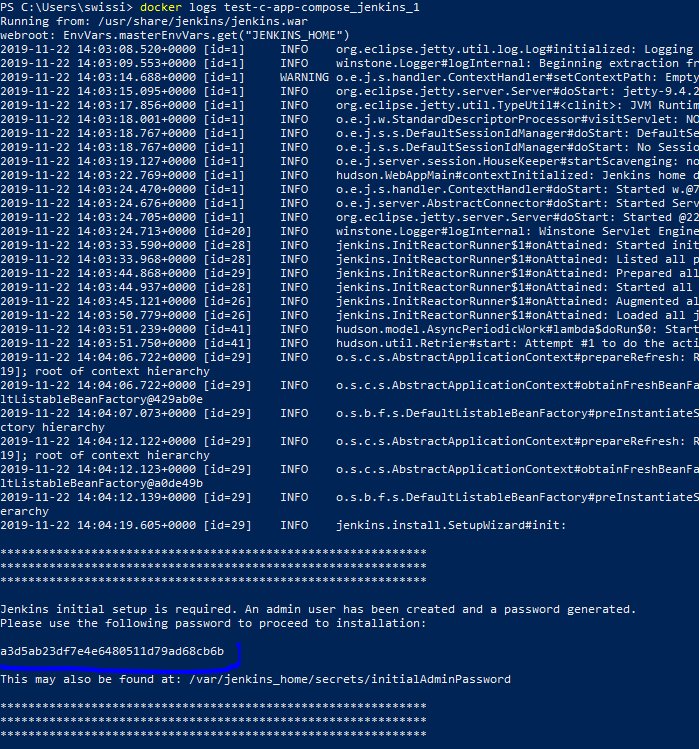
\includegraphics[width=15cm, height=17cm]{jenkins-logs.PNG}
		\caption{Container Logs} 
		\label{Container Logs} 
	\end{center}
\end{figure}
\newpage
Nach dem Entsperren von Jenkins wird die Seite 'Customize-Jenkins' angezeigt. Hier können Sie im Rahmen Ihrer Ersteinrichtung beliebig viele nützliche Plugins installieren.

\begin{figure}[h!]
	\begin{center}
		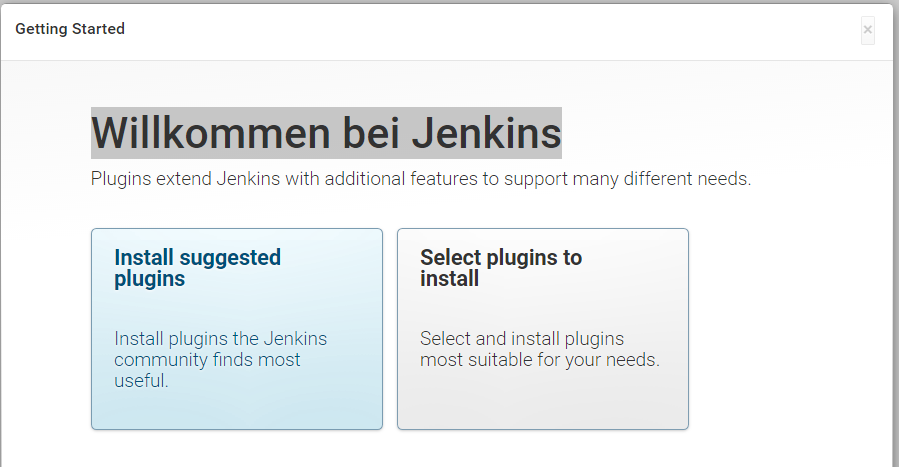
\includegraphics[width=17cm, height=6cm]{customize-jenkins.PNG}
		\caption{Jenkins entsperren Seite} 
		\label{Jenkins entsperren Seite} 
	\end{center}
\end{figure}


Klicken Sie auf eine der beiden angezeigten Optionen:
\begin{itemize}
	\item \textbf{Install suggested plugins: } Um die empfohlenen Plugins zu installieren, die auf den häufigsten Anwendungsfällen basieren.
	\item \textbf{Select plugins to install}um auszuwählen, welche Plugins zuerst installiert werden sollen. Wenn Sie zum ersten Mal auf die Plugin-Auswahlseite zugreifen, werden standardmäßig die vorgeschlagenen Plugins ausgewählt.
\end{itemize}
Der Setup-Assistent zeigt den Fortschritt der Konfiguration von Jenkins und die Installation der ausgewählten Jenkins-Plugins an. Dieser Vorgang kann einige Minuten dauern.
\newline
Nachdem Sie Jenkins mit Plugins angepasst haben, werden Sie von Jenkins aufgefordert, Ihren ersten Administratorbenutzer zu erstellen.
\begin{itemize}
	\item Geben Sie auf der Seite Create First Admin User (Erster Administratorbenutzer erstellen) die Details für Ihren Administratorbenutzer in die entsprechenden Felder ein und klicken Sie auf Save and Finish (Speichern und Fertig stellen).
	\item Wenn die Seite 'Jenkins is ready' angezeigt wird, klicken Sie auf 'Start using Jenkins'.
\end{itemize}

\section{Verwendung}
In diesem Abschnitt wird die Verwendung der Test C-Plattform erläutert.
\subsection{Admin-Portal}
Der Administrator meldet sich zuerst über die Anmeldeseite an.
\begin{figure}[h!]
	\begin{center}
		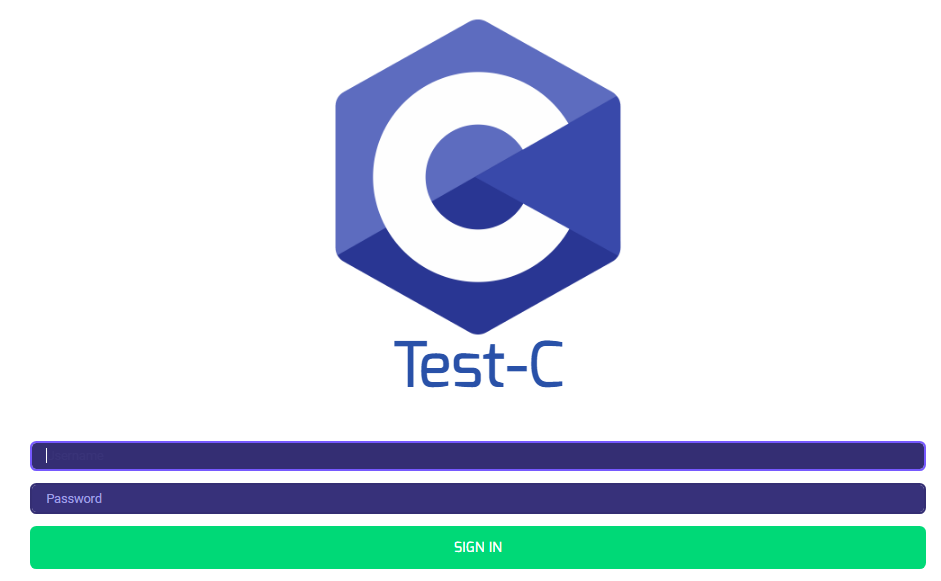
\includegraphics[width=14cm, height=5cm]{AdminLogin.PNG}
		\caption{Login Seite} 
		\label{Login Seite} 
	\end{center}
\end{figure}
\newline
Nach der Anmeldung kann der Administrator die folgenden Dienste verwenden:
\paragraph{Add-Aufgabenblatt: }Erstellung eines Testbereichs für das neue Aufgabenblatt.
\newline
Zunächst muss der Administrator über die Gogs-Oberfläche ein Remote-Git-Repository für das Aufgabenblatt erstellen.
\begin{figure}[h!]
	\begin{center}
		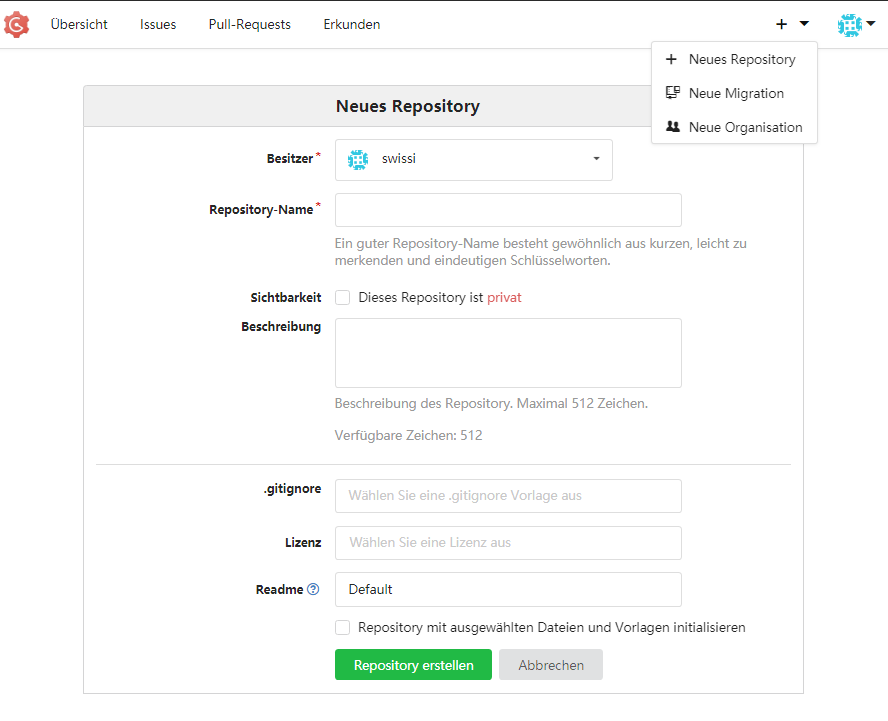
\includegraphics[width=12cm, height=9cm]{Aufgabenblatt-Git-Repo.PNG}
		\caption{Erstellung eines Remote-Git-Repository} 
		\label{Erstellung eines Remote-Git-Repository} 
	\end{center}
\end{figure}
\newpage
Anschließend wendet sich der Administrator an Admin Portal FrontEnd, um die Erstellung des Arbeitsblatts abzuschließen.
\begin{figure}[h!]
	\begin{center}
		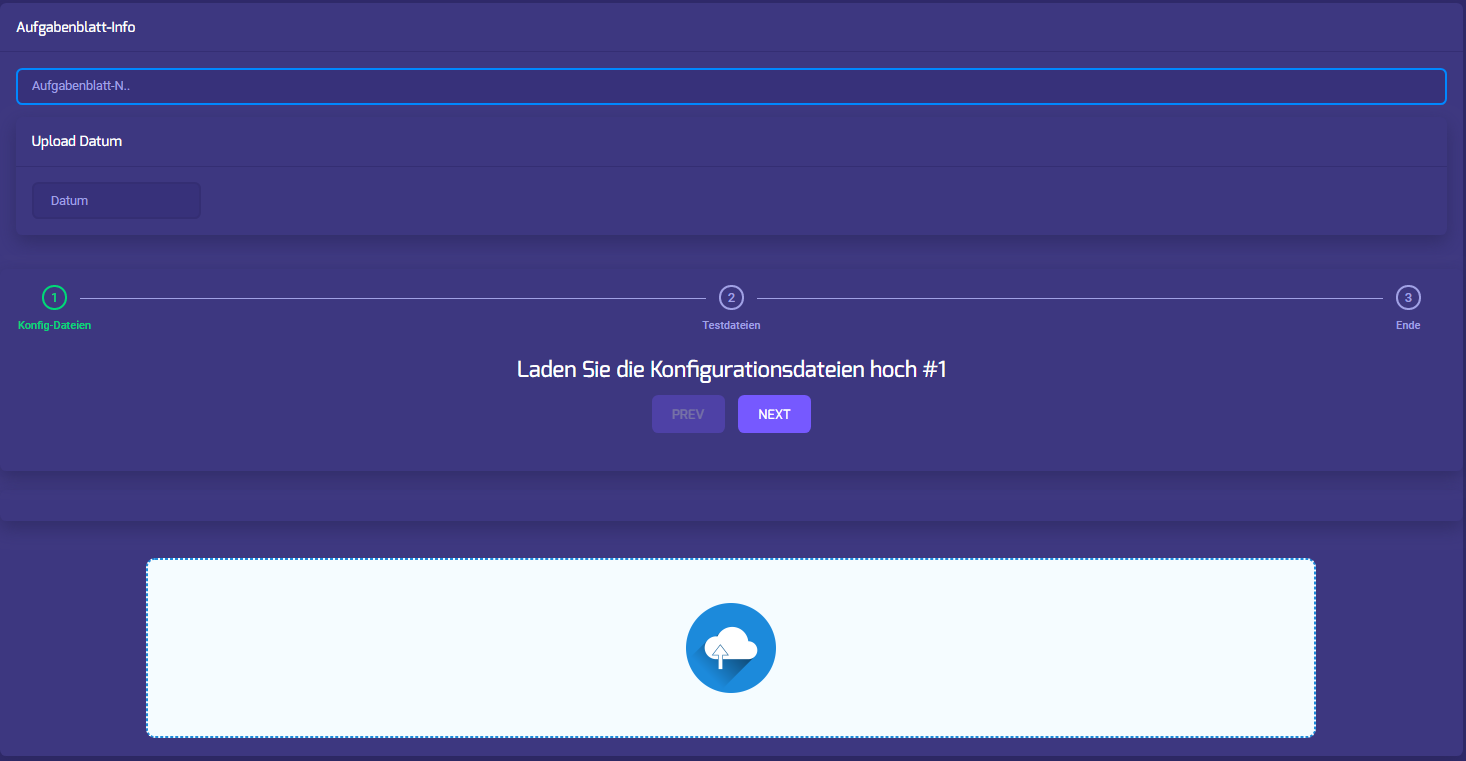
\includegraphics[width=16cm, height=10cm]{Add-Aufgabenblatt.PNG}
		\caption{Add-Aufgabenblatt} 
		\label{Add-Aufgabenblatt} 
	\end{center}
\end{figure}
\newline
Der Administrator schreibt zuerst den Namen des Aufgabenblatts, das er erstellen möchte.Anschließend werden die für den Testprozess erforderlichen Dateien hochgeladen. Dieser Vorgang erfolgt in zwei Schritten:
\begin{itemize}
	\item Hochladen von Konfigurationsdateien (makefile und jenkinsfile).
	\item Hochladen von Testdateien 
\end{itemize}
\newpage
\paragraph{Aufgabenblatt Anzeigen: } Auf der Seite 'Augabenblaetter' kann der Administrator die erstellten Aufgabenblätter anzeigen und die gewünschte Datei löschen.
\begin{figure}[h!]
	\begin{center}
		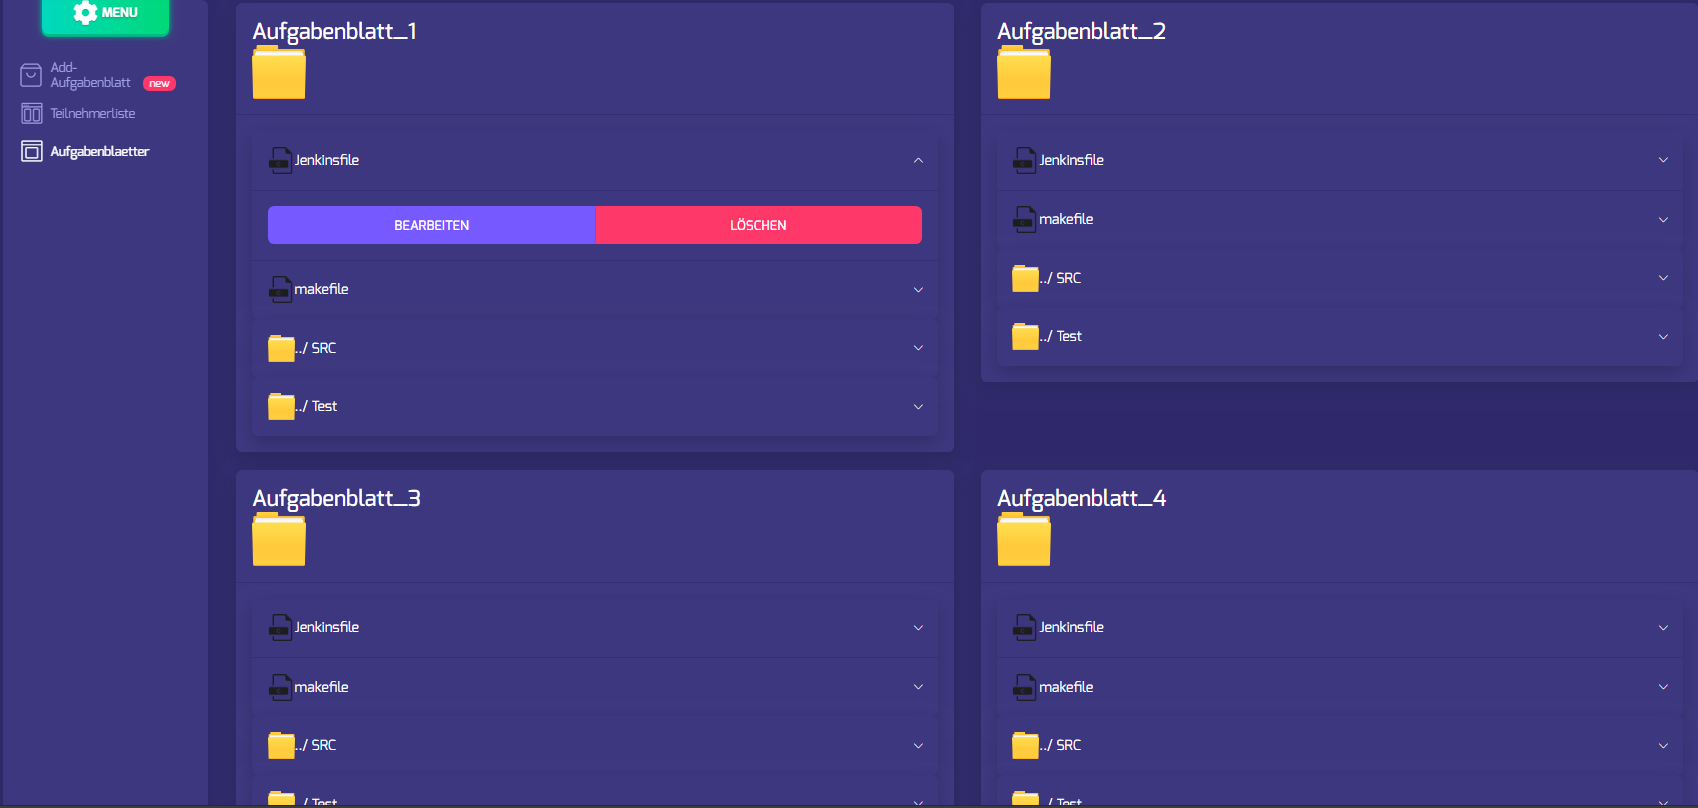
\includegraphics[width=18cm, height=14cm]{aufgabenblaetter.PNG}
		\caption{Augabenblätter anzeigen} 
		\label{Augabenblätter anzeigen} 
	\end{center}
\end{figure}
\newpage
\subsection{Studenten-Portal}
Der Student meldet sich zuerst über die Anmeldeseite an. Anschließend kann er die zu testende Datei über die Seite 'Add-Aufgabenblatt-Lösung' hochladen.
\newline
Achtung: Bitte vergessen Sie nicht, den Namen des zu testenden Aufgabenblatts einzugeben.
\begin{figure}[h!]
	\begin{center}
		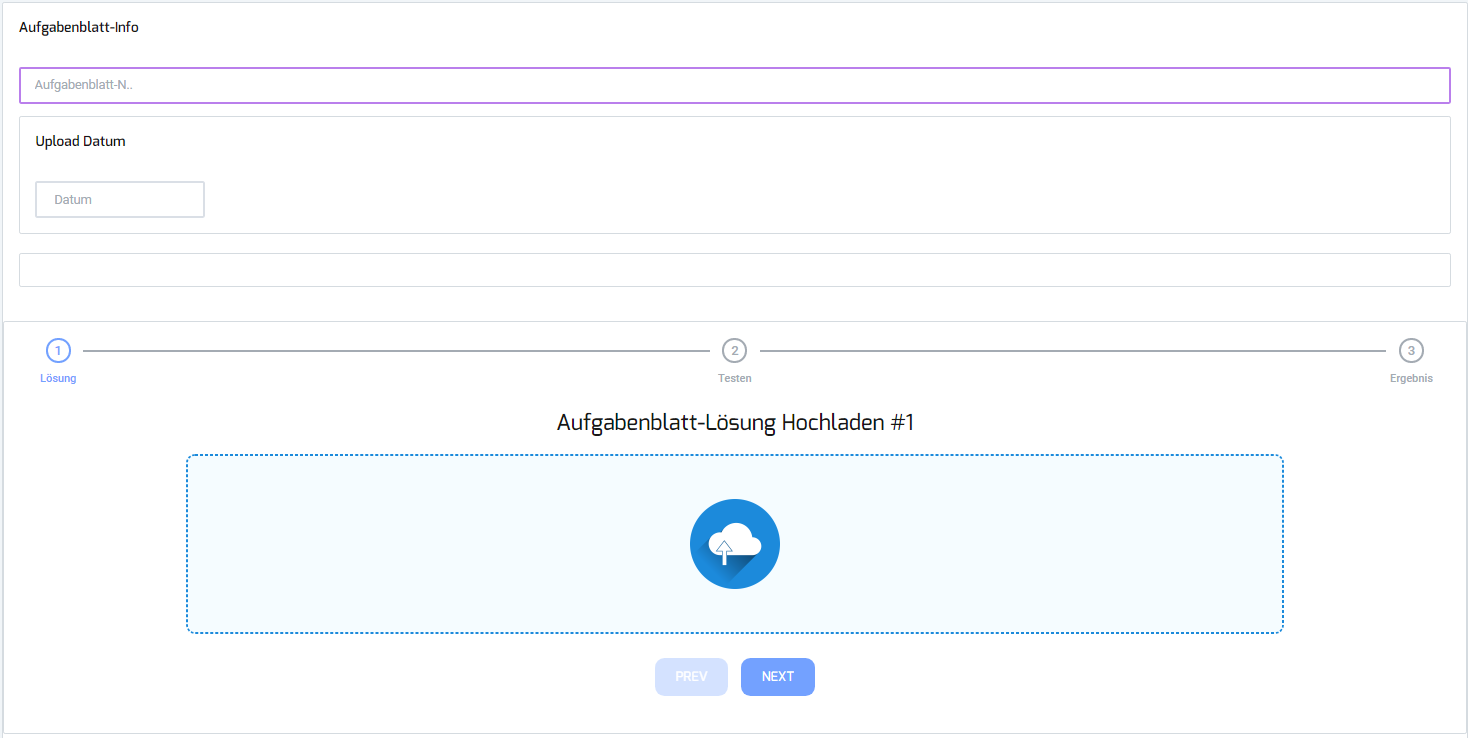
\includegraphics[width=16cm, height=8cm]{Add-Aufgabenblatt-Loesung.PNG}
		\caption{Add-Aufgabenblatt-Lösung} 
		\label{Add-Aufgabenblatt-Lösung} 
	\end{center}
\end{figure}
\newline
Nach dem Hochladen der Datei kann der Benutzer den Befehl zum Starten des Testprozesses absetzen.
\begin{figure}[h!]
	\begin{center}
		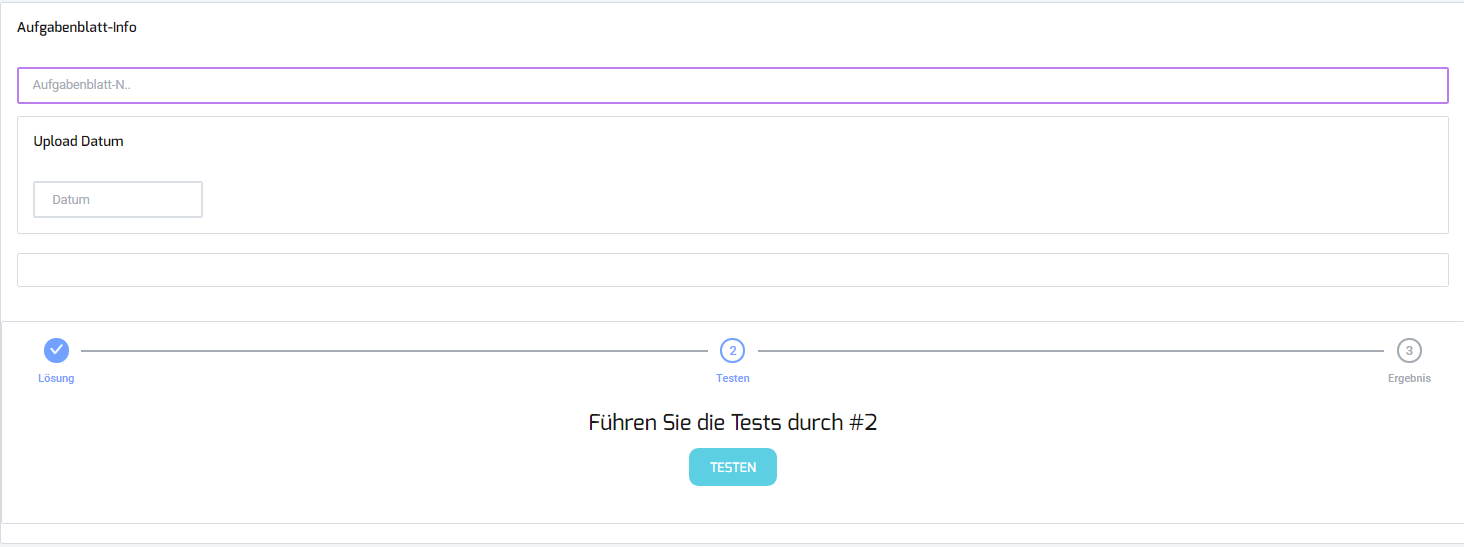
\includegraphics[width=16cm, height=6cm]{tests-fuehren.PNG}
		\caption{Add-Aufgabenblatt-Lösung} 
		\label{Add-Aufgabenblatt-Lösung} 
	\end{center}
\end{figure}
\newpage
Nach einer kurzen Wartezeit wird dem Benutzer das Testergebnis angezeigt.
\begin{figure}[h!]
	\begin{center}
		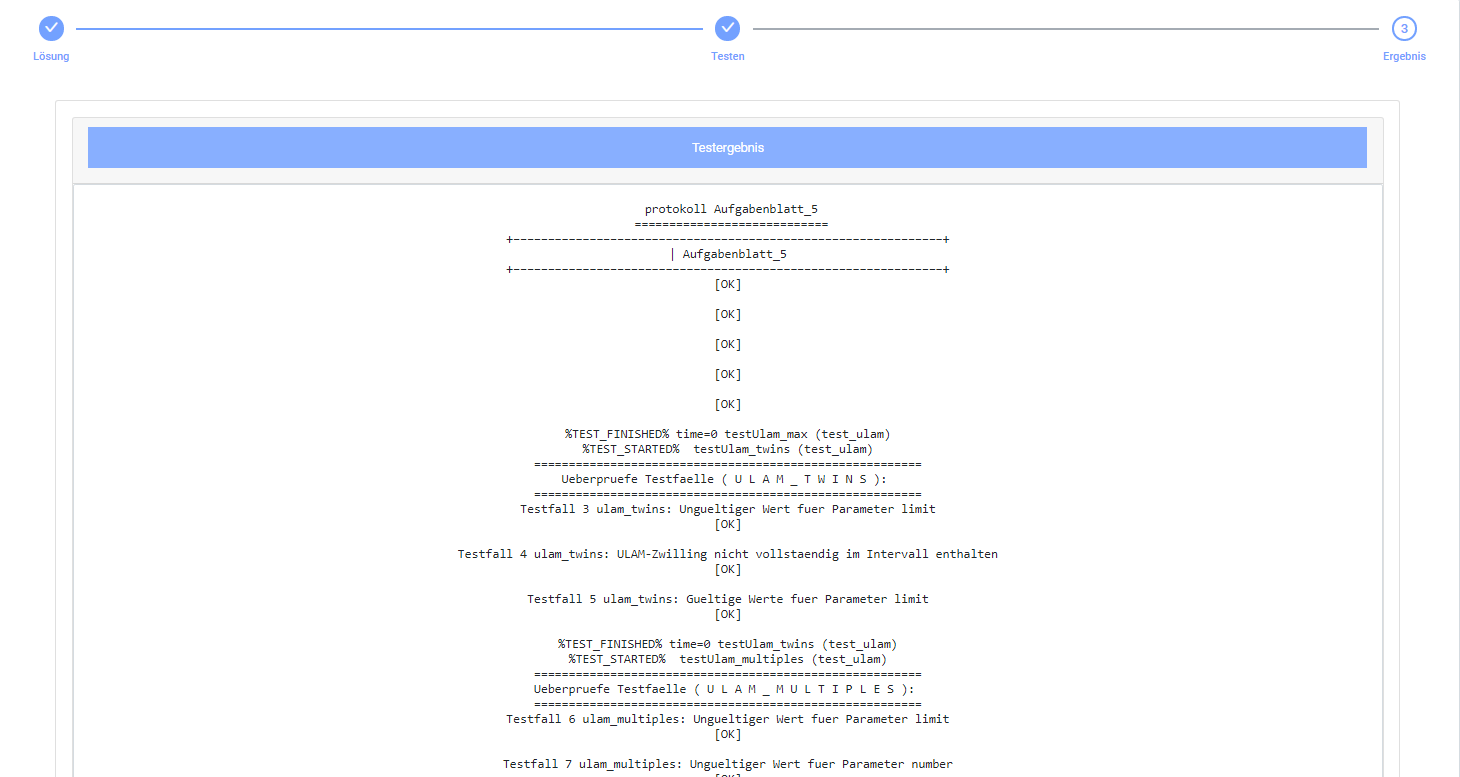
\includegraphics[width=16cm, height=16cm]{Testergebnis.PNG}
		\caption{Testergebnis} 
		\label{Testergebnis} 
	\end{center}
\end{figure}
\chapter{Zusammenfassung}
\addcontentsline{toc}{chapter}{Literaturverzeichnis}
\begin{thebibliography}{9}
\end{thebibliography}
\end{document}